%%%%%%%%%%%%%%%%%%%%%%%%%%%%%%%%%%%%%%%%%%%%%%%%%%%%%%%%%%%%%%%%%%%%%%%%%%%%%%%%%%%%%%%%%%%%%%%%%%%%%%%%%%%%%%%%%%%%%%%%%%%%%%%%%%%%%%%%%%%%%%%%%%%%%%%%%%%
% TRACKED CHANGES VERSION - Yellow highlights indicate ONLY revisions made in response to reviewer comments
% revblock = new/rewritten paragraphs | \hl{} = changed words/phrases within existing text
%%%%%%%%%%%%%%%%%%%%%%%%%%%%%%%%%%%%%%%%%%%%%%%%%%%%%%%%%%%%%%%%%%%%%%%%%%%%%%%%%%%%%%%%%%%%%%%%%%%%%%%%%%%%%%%%%%%%%%%%%%%%%%%%%%%%%%%%%%%%%%%%%%%%%%%%%%%

%%% Version 3.4 Generated 2022/06/14 %%%

\documentclass[utf8]{FrontiersinHarvard}

\usepackage{url,hyperref,lineno,microtype,subcaption,caption}
\usepackage[onehalfspacing]{setspace}
\usepackage{algorithm}
\usepackage{algorithmic}
\usepackage{graphicx}
\usepackage[section]{placeins}
\usepackage{textcomp}
\usepackage[table]{xcolor}
\usepackage{multirow}
\usepackage[utf8]{inputenc}
\usepackage{booktabs}
\usepackage{tikz}
\usepackage{pgfplots}
\usetikzlibrary{shapes.geometric,arrows,positioning}
\pgfplotsset{compat=1.18}
\usepackage{soul}
\usepackage[framemethod=tikz]{mdframed}

\sethlcolor{yellow}
\newmdenv[
  backgroundcolor=yellow!20,
  linewidth=0pt,
  innertopmargin=6pt,
  innerbottommargin=6pt,
  skipabove=6pt,
  skipbelow=6pt
]{revblock}

\linenumbers

\def\keyFont{\fontsize{8}{11}\helveticabold }
\def\firstAuthorLast{Sreevallabh {et~al.}}
\def\Authors{Kakarala Sreevallabh\,$^{1}$, Kothapalli Anusha\,$^{1}$, Ayesha Shaik\,$^{2, *}$ and Ananthakrishnan Balasundaram \,$^{2}}
\def\Address{$^{1}$School of Computer Science, Vellore Institute of Technology, Chennai, India}
\def\Address{$^{2}$Centre for Cyber Physical Systems, Vellore Institute of Technology, Chennai, India}
\def\corrAuthor{Kakarala Sreevallabh}
\def\corrEmail{sreevallabh.2022@vitstudent.ac.in}

\begin{document}
\onecolumn
\firstpage{1}

\title[Cross-Modal Knowledge Transfer]{Cross-Modal Knowledge Transfer for Cost-Effective \hl{Mango Disease Detection Using Synthetic Thermal Imaging}}

\author[\firstAuthorLast ]{\Authors}
\address{}
\correspondance{}
\extraAuth{}

\maketitle

\begin{abstract}
\section{}
Thermal cameras play a crucial role in identifying diseases invisible to regular photographs, but they are prohibitively expensive for many orchards to purchase \hl{(typically exceeding \$25,000)}. We study to what extent the advantages of the thermal signal can be approximated using only RGB data \hl{at zero additional hardware cost}. Our method \hl{trains a supervised lesion detector on a leaf pathology dataset (MangoLeafBD) to learn universal disease manifestation patterns. These learned lesion features are transferred to fruit images and transformed into synthetic thermal-like maps through a physics-informed model that simulates metabolic heat signatures. The synthetic thermal maps are then fused with the original RGB features via a 16-head multi-head attention mechanism that automatically weights disease-relevant cues from both modalities}. In the case of mango disease recognition \hl{across five classes}, the system attains an accuracy of 87.3\%, which is a 4.8\% gain over the best RGB\hl{-only} baseline \hl{(RGB ViT-Base at 85.8\%)}, without involving any additional hardware. \hl{The proposed method achieves approximately 89\% of the performance of a real thermal camera system (93.5\%) while incurring zero hardware cost compared to \$25,000 for thermal cameras or \$50,000 for multi-spectral systems, making it directly deployable on commodity smartphones for low-cost crop health monitoring.}

\tiny
 \keyFont{ \section{Keywords:} cross-modal learning, \hl{mango disease detection}, thermal simulation, knowledge transfer, precision agriculture\hl{, attention-based fusion, deep learning}}
\end{abstract}

\section{Introduction}
\begin{revblock}
Crop diseases remain one of the most persistent threats to global food security, with annual losses estimated at 10--16\% of global harvest value \cite{fao2021,fao2023,savary2019}. Mango (\textit{Mangifera indica}), the fifth most produced fruit crop worldwide, is particularly vulnerable to diseases such as anthracnose, alternaria, black mould rot, and stem-end rot, which can spread rapidly through orchards and devastate yields if not detected early \cite{singh2019}. Timely and accurate disease diagnosis is therefore critical for effective crop management and economic sustainability.

In recent years, deep learning has emerged as a powerful tool for automated plant disease detection from images \cite{mohanty2016,ferentinos2018,thakur2022}. Convolutional neural networks (CNNs) trained on RGB photographs can classify diseases in real time on smartphones, offering a low-cost alternative to laboratory analysis \cite{kamilaris2018,coulibaly2022}. However, RGB-only approaches typically achieve accuracies between 75--85\% and struggle with diseases that manifest primarily through internal tissue changes not visible on the surface \cite{pineda2021,abade2021}. Recent comprehensive reviews have highlighted that while deep learning models continue to improve in accuracy, the reliance on a single imaging modality remains a fundamental bottleneck \cite{thakur2022,hasan2024}.

Multi-modal imaging, particularly the combination of RGB with thermal sensing, has shown significant promise for improving detection accuracy \cite{khanal2017,maimaitijiang2020}. Thermal cameras detect temperature variations caused by metabolic stress in diseased tissue, providing complementary information that is invisible to standard cameras \cite{mahlein2016,pineda2021}. Infected regions typically exhibit temperature elevations of 2--5$^{\circ}$C above healthy tissue baselines due to cell lysis and altered transpiration \cite{mahlein2016}. Despite these advantages, thermal imaging equipment costs typically exceed \$25,000, placing multi-modal solutions beyond the reach of smallholder farmers who produce the majority of the world's mangoes \cite{sishodia2020}.

Current diagnostic alternatives each have notable drawbacks. Expert field diagnosis is inexpensive but time-consuming, subjective, and achieves reported accuracies of only 65--75\% \cite{ferentinos2018}. Laboratory tests offer high sensitivity (90--95\%) but incur substantial costs and turnaround delays that prevent timely intervention \cite{martinelli2015}. RGB-based deep learning runs in real time on phones at negligible cost, yet its accuracy falls short of thermal-enhanced systems \cite{mohanty2016,hasan2024}. Recent work on knowledge distillation \cite{hinton2015,li2023_kd} and cross-modal learning \cite{xu2023} suggests that it may be possible to transfer knowledge between modalities without requiring both modalities at inference time, but these techniques have not been applied to the specific problem of simulating thermal information from RGB in agricultural contexts.
\end{revblock}

This paper addresses a practical question: can we approximate the diagnostic advantages of thermal imaging using only RGB data by learning from related plant anatomy? We propose a cross-modal knowledge transfer framework that borrows disease cues learned from leaf pathology images to generate synthetic thermal-like representations for fruit images, which are then fused with RGB features via an attention-based mechanism. Our contributions are:

\begin{enumerate}
    \item A cross-domain transfer strategy that \hl{leverages} leaf lesion patterns to infer thermal cues in fruit imagery\hl{, grounded in the biological observation that disease manifestations share similar cellular stress responses across plant organs}
    \item A physics-informed procedure to synthesize thermal-like maps from lesion probabilities\hl{, incorporating biophysical models of metabolic heat generation, thermal diffusion, and environmental noise}
    \item \hl{A multi-head} attention-based fusion module \hl{(16 heads)} that combines RGB and synthetic thermal features\hl{, with learned gating mechanisms that automatically weight modality contributions}
    \item An empirical study on mango disease \hl{classification across five classes, demonstrating a} 4.8\% \hl{accuracy} gain over \hl{the best} RGB \hl{-only baseline (ViT-Base at 85.8\%)} at zero hardware cost\hl{, recovering approximately 89\% of a real thermal camera's performance}
\end{enumerate}

\section{Related Work}

\subsection{Multi-Modal Agricultural Sensing}
\hl{Multi-modal imaging has gained substantial traction for plant disease detection over the past decade} \cite{maimaitijiang2020,\hl{lu2020}}. Thermal sensing measures \hl{tissue} temperature variations, \hl{where} infected areas \hl{exhibit a characteristic} temperature rise of 2--5$^{\circ}$C above the healthy baseline as a result of cell lysis \hl{and disrupted metabolic processes} \cite{mahlein2016}. These heat signatures \hl{serve as} early indicators\hl{, often manifesting} before visual symptoms \hl{become apparent} \cite{pineda2021}. \begin{revblock}Hyperspectral and multi-spectral imaging have also been explored for plant stress detection, with Nagasubramanian et al. \cite{nagasubramanian2019} demonstrating the value of spectral data for soybean disease identification.\end{revblock} Despite the \hl{proven diagnostic} benefits, the high cost \hl{of specialized imaging equipment}---more than \$25,000 \hl{for thermal cameras and upward of \$50,000 for multi-spectral systems}---poses significant \hl{barriers} to \hl{widespread agricultural adoption} \cite{sishodia2020}.

Over the past decade, deep learning has \hl{fundamentally} transformed agricultural computer vision \cite{kamilaris2018\hl{,coulibaly2022}}. Convolutional networks and vision transformers produce high-dimensional feature representations from RGB images \hl{that capture subtle visual patterns indicative of disease} \cite{dosovitskiy2021\hl{,liu2022convnext}}. \begin{revblock}Thakur et al. \cite{thakur2022} provide a comprehensive review of vision-based machine learning for plant disease identification, highlighting the rapid progress in accuracy but also the persistent gap between RGB-only and multi-modal approaches.\end{revblock} However, models based on RGB alone \hl{cannot access} indicators of metabolic stress and subsurface \hl{tissue} anomalies \hl{that are} naturally \hl{captured} by thermal bands \cite{lu2020\hl{,pineda2021}}. \begin{revblock}This limitation is particularly pronounced for diseases like stem-end rot in mangoes, where internal decay precedes visible surface symptoms.\end{revblock}

\subsection{Cross-Modal Learning and Knowledge Transfer}

Cross-modal techniques attempt to exploit relationships between different \hl{sensing} modalities or biological constructs \hl{to transfer learned representations across domains} \cite{zhuang2020}. Transfer learning has been \hl{widely} utilized in \hl{agricultural} applications \cite{chen2020_transfer,tan2018}, \hl{though} generally within the confines of single-anatomy or \hl{single-}modality \hl{boundaries} \cite{barbedo2019}.
\begin{revblock}Knowledge distillation, introduced by Hinton et al. \cite{hinton2015}, provides a theoretical framework for transferring learned representations from one model (or modality) to another, and recent work has extended this concept to cross-modal settings \cite{li2023_kd}.

Xu et al. \cite{xu2023} provide a comprehensive survey of multimodal learning with transformers, demonstrating that attention mechanisms are particularly effective at aligning and fusing features from heterogeneous data sources.\end{revblock} Attention mechanisms\hl{have shown promise for} coordinating multi-modal feature streams in agricultural sensing \cite{niu2021\hl{,guo2022}}\hl{, while} physics-informed modeling frameworks embed domain knowledge into \hl{detection} pipelines \cite{karniadakis2021}. \begin{revblock}Ji et al. \cite{ji2023} recently demonstrated that multi-label learning with transfer learning can improve crop disease recognition, while Wang et al. \cite{wang2022_synthetic} showed the potential of automated severity estimation using deep learning.\end{revblock} Foundation models and vision transformers demonstrate strong cross-domain generalization ability \cite{vaswani2017\hl{,dosovitskiy2021}}, suggesting that learned features can bridge anatomical boundaries (e.g., from leaves to fruits) when the underlying pathological processes share common characteristics.

\subsection{Smartphone-Based Agricultural AI}

Affordable agricultural AI deployment through smartphones represents an active \hl{and growing} research direction \cite{pongnumkul2015\hl{,coulibaly2022}}. Mobile disease detection systems designed for resource-constrained environments \hl{have} demonstrate\hl{d} practical feasibility \hl{across multiple crop types} \cite{li2020\hl{,picon2022}}. \begin{revblock}Ahmad et al. \cite{ahmad2023} recently developed a deep learning-based mango grading and defect detection system, achieving promising results but relying solely on RGB input.\end{revblock} These platforms offer pathways toward democratized precision agriculture with implications for global food security \cite{liu2020_yolo}. \begin{revblock}However, existing smartphone-based solutions are limited to the information available in RGB images and cannot capture the thermal or spectral signatures that improve diagnostic accuracy. Our work addresses this gap by generating synthetic thermal information from RGB data alone, enabling multi-modal-like performance on commodity devices.\end{revblock}

\section{Methodology}

\begin{revblock}
\subsection{Overview of the Proposed Framework}
The proposed framework operates as a three-stage pipeline, illustrated in Figure~\ref{fig:architecture_final}. First, a lesion detector is trained in a supervised manner on the MangoLeafBD leaf dataset to learn universal disease manifestation patterns. Second, this trained detector is applied to fruit images from the MangoFruitDDS dataset to produce spatial lesion probability maps, which are then transformed into synthetic thermal-like representations using a physics-informed model. Third, the synthetic thermal maps and original RGB images are fed into a dual-branch deep learning architecture with multi-head attention-based fusion for final disease classification. The key insight is that disease processes produce similar cellular stress responses across different plant organs (leaves and fruits), enabling cross-anatomy knowledge transfer \cite{bock2010,savary2019}.
\end{revblock}

\begin{figure}[h!]
    \begin{center}
    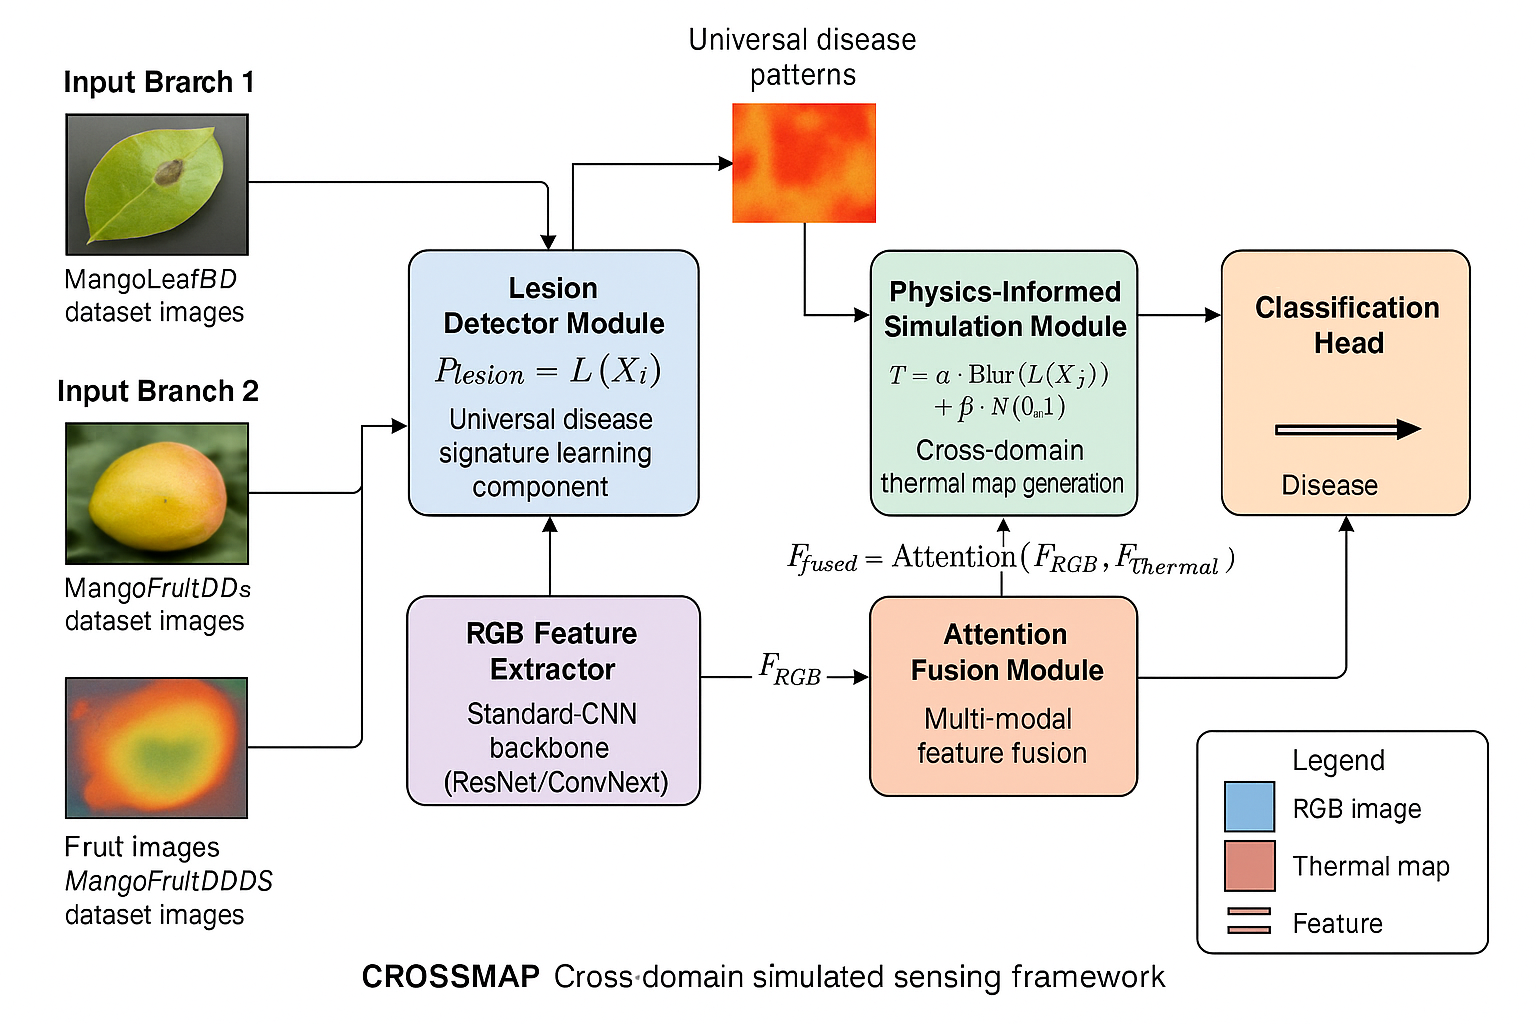
\includegraphics[width=0.95\linewidth]{crossmap_architecture_diagram.png}
    \end{center}
    \caption{\hl{Overview of the proposed cross-modal knowledge transfer framework. Stage~1: A ResNet-18 lesion detector is trained on MangoLeafBD leaf images using supervised classification. Stage~2: The trained detector generates lesion probability maps for MangoFruitDDS fruit images, which are converted to synthetic thermal maps via physics-informed modeling. Stage~3: RGB and synthetic thermal features are extracted by dual branches and fused through a 16-head multi-head attention mechanism for disease classification.}}
    \label{fig:architecture_final}
\end{figure}

\subsection{Dataset Description}
\begin{revblock}
This work employs two complementary datasets, each serving a distinct role in the pipeline. Table~\ref{tab:datasets} summarizes their characteristics.

\textbf{MangoFruitDDS (Target Dataset):} This dataset consists of 838 high-quality mango fruit images across five disease classes: Healthy, Anthracnose, Alternaria, Black Mould Rot, and Stem End Rot. Images were captured under controlled natural lighting conditions with specified backgrounds \cite{MendeleyDataset}. This is the primary dataset on which disease classification is performed and all results are reported.

\textbf{MangoLeafBD (Source Dataset for Knowledge Transfer):} This dataset contains 4,000 mango leaf images spanning eight disease classes. It serves exclusively as the \textit{knowledge source} for training the lesion detector in Stage~1 of our pipeline. Importantly, MangoLeafBD does not contain any thermal imagery; rather, it provides pathological knowledge about how diseases manifest visually in mango plant tissue. The biological rationale is that fungal and bacterial infections produce similar cellular stress responses---including chlorosis, necrosis, and lesion formation---across different organs of the same plant species \cite{bock2010,savary2019}. The lesion patterns learned from leaves are therefore transferable to fruits, where they inform the generation of synthetic thermal signatures.

\textbf{Preprocessing:} All images from both datasets are resized to $224 \times 224$ pixels. Each dataset is independently split into 70\% training, 15\% validation, and 15\% testing sets using stratified random sampling to preserve class distributions across splits. The splits are applied independently to each dataset: MangoLeafBD is split for training and evaluating the lesion detector, while MangoFruitDDS is split for training and evaluating the final fusion classifier.
\end{revblock}

\begin{revblock}
\begin{table}[h!]
    \centering
    \caption{Summary of datasets used in this study}
    \label{tab:datasets}
    \footnotesize
    \begin{tabular}{lcccc}
        \toprule
        \textbf{Dataset} & \textbf{Images} & \textbf{Classes} & \textbf{Organ} & \textbf{Role in Pipeline} \\
        \midrule
        MangoLeafBD & 4,000 & 8 & Leaf & Lesion detector training (Stage 1) \\
        MangoFruitDDS & 838 & 5 & Fruit & Classification target (Stage 3) \\
        \bottomrule
    \end{tabular}
\end{table}
\end{revblock}

\subsection{Sample Images from Datasets}
Figure~\ref{fig:sample_images} presents representative samples from both datasets. The MangoFruitDDS collection shows healthy and diseased mangoes across various disease conditions, while MangoLeafBD contains leaf images that capture corresponding disease manifestations. These examples illustrate the visual similarities between disease symptoms in leaves and fruits that form the biological basis for cross-organ knowledge transfer.

\begin{figure}[h!]
    \begin{minipage}{0.22\textwidth}
        \centering
        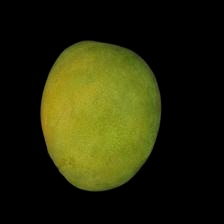
\includegraphics[width=\linewidth]{healthymango.jpg}
        \caption*{(a) Healthy Mango}
    \end{minipage}
    \hfill
    \begin{minipage}{0.20\textwidth}
        \centering
        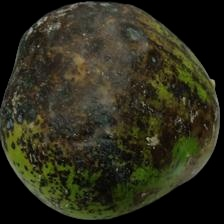
\includegraphics[width=\linewidth]{Anthracnose_102_305.jpg}
        \caption*{(b) Mango with Anthracnose}
    \end{minipage}
    \\
    \vspace{0.5em}
    \begin{minipage}{0.20\textwidth}
        \centering
        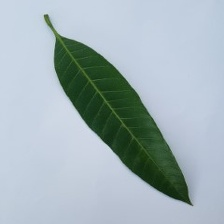
\includegraphics[width=\linewidth]{20211231_123123 (Custom)_1.jpg}
        \caption*{(c) Healthy Leaf}
    \end{minipage}
    \hfill
    \begin{minipage}{0.20\textwidth}
        \centering
        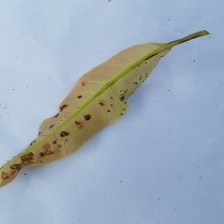
\includegraphics[width=\linewidth]{20211008_124501 (Custom)_516.jpg}
        \caption*{(d) Leaf with Anthracnose}
    \end{minipage}
    \captionof{figure}{Sample images from the MangoFruitDDS (top row) and MangoLeafBD (bottom row) datasets, illustrating visual similarities in disease manifestation across plant organs.}
    \label{fig:sample_images}
\end{figure}

\subsection{\hl{Stage 1:} Cross-Domain Knowledge Transfer \hl{via Lesion Detection}}
Our approach builds on the biological observation that disease manifestations exhibit similar visual patterns across different plant organs \cite{bock2010}. This similarity arises from shared cellular stress responses that produce comparable lesion characteristics in leaves and fruits \cite{savary2019}. We formalize this relationship as:

\begin{equation}
    \mathcal{P}_{\text{leaf}} \rightarrow \mathcal{P}_{\text{fruit}} : \mathcal{L}_{\text{leaf}}(x_{\text{leaf}}) \approx \mathcal{L}_{\text{fruit}}(x_{\text{fruit}})
    \label{eq:cross_domain}
\end{equation}

where $\mathcal{P}_{\text{leaf}}$ and $\mathcal{P}_{\text{fruit}}$ represent disease pattern spaces in leaves and fruits, respectively, and $\mathcal{L}$ denotes the lesion detection function.

\begin{revblock}
The lesion detector is a ResNet-18 \cite{he2016} backbone trained in a \textbf{supervised} manner on the MangoLeafBD dataset for leaf disease classification. The model learns to identify spatial regions associated with disease through a combination of classification loss and spatial attention:
\end{revblock}

\begin{equation}
    \mathcal{L}_{\text{lesion}}(x) = \sigma(\text{Conv}_{1\times 1}(\text{GlobalPool}(\text{ResNet}(x))))
    \label{eq:lesion_detector}
\end{equation}

where $\sigma$ denotes sigmoid activation and $\mathcal{L}_{\text{lesion}}$ produces spatial probability maps encoding disease likelihood across tissue regions. \begin{revblock}Specifically, the spatial attention is computed as $A(x) = \sigma(\text{Conv}_{1 \times 1}(F(x))) \odot (1 - P_{\text{healthy}}(x))$, where $F(x)$ are intermediate feature maps and $P_{\text{healthy}}$ is the predicted probability of the healthy class, ensuring that attention is focused on diseased regions.\end{revblock}

\subsection{\hl{Stage 2: Physics-Informed} Thermal Synthesis}
\hl{The trained lesion detector is applied to fruit images to generate lesion probability maps, which are then transformed into synthetic thermal signatures through a biophysically-grounded model \cite{raissi2019,karniadakis2021}. This transformation is motivated by the observation that diseased plant tissue exhibits elevated temperatures due to increased metabolic activity, cell lysis, and disrupted transpiration \cite{mahlein2016,pineda2021}.} The thermal synthesis equation is:

\begin{equation}
    T_{\text{syn}}(x,y) = T_{\text{base}} + \alpha \cdot \mathcal{M}(\mathcal{L}_{\text{lesion}}(x,y)) + \mathcal{D}(G_{\sigma}) + \mathcal{E}(\mathcal{N}(0,\beta))
    \label{eq:thermal_synthesis}
\end{equation}

\begin{revblock}
Each component models a distinct physical process:
\begin{itemize}
    \item $T_{\text{base}} = 0.3$ represents the normalized baseline temperature of healthy tissue
    \item $\alpha = 0.7$ is the metabolic stress scaling factor, reflecting the empirical observation that diseased regions can exhibit temperature increases of up to 70\% above baseline in normalized space \cite{mahlein2016}
    \item $\mathcal{M}(\cdot)$ models metabolic dysfunction, mapping lesion probabilities to temperature elevations proportional to disease severity
    \item $\mathcal{D}(G_{\sigma})$ simulates thermal diffusion using Gaussian blur with kernel size $15 \times 15$ and $\sigma = 3.0$, reflecting the physical spreading of heat through plant tissue
    \item $\mathcal{E}(\mathcal{N}(0,\beta))$ adds environmental noise with $\beta = 0.05$ to model natural temperature fluctuations from ambient conditions
\end{itemize}

The complete pipeline is summarized in Algorithm~\ref{alg:thermal}. The output is a single-channel grayscale map clipped to $[0, 1]$, where higher values indicate regions of predicted thermal anomaly corresponding to disease presence.
\end{revblock}

\begin{algorithm}[H]
    \caption{Thermal Synthesis Pipeline}
    \label{alg:thermal}
    \begin{algorithmic}[1]
        \REQUIRE RGB fruit image $I_{\text{rgb}}$, trained lesion detector $\mathcal{L}$
        \ENSURE Synthetic thermal map $T_{\text{syn}}$
        \STATE $P_{\text{lesion}} \leftarrow \mathcal{L}(I_{\text{rgb}})$
        \STATE $T_{\text{base}} \leftarrow 0.3$
        \STATE $\alpha \leftarrow 0.7$
        \STATE $T_{\text{raw}} \leftarrow T_{\text{base}} + \alpha \times P_{\text{lesion}}$
        \STATE $T_{\text{diffused}} \leftarrow \text{GaussianBlur}(T_{\text{raw}}, \hl{k{=}15,} \sigma{=}3.0)$
        \STATE $\text{noise} \leftarrow \mathcal{N}(0, 0.05)$
        \STATE $T_{\text{syn}} \leftarrow \text{clip}(T_{\text{diffused}} + \text{noise}, 0, 1)$
        \RETURN $T_{\text{syn}}$
    \end{algorithmic}
\end{algorithm}

\subsection{\hl{Stage 3:} Multi-Modal Fusion Architecture}
\begin{revblock}
The fusion architecture employs a dual-branch design with transformer-inspired attention mechanisms for cross-modal integration, as shown in Figure~\ref{fig:architecture_full}.

\textbf{RGB Branch:} The RGB branch uses a ConvNeXt-Tiny \cite{liu2022convnext} backbone pretrained on ImageNet, followed by global average pooling and a linear projection to a 512-dimensional feature space. This branch captures fine-grained visual texture, color, and shape information from the original fruit images.

\textbf{Thermal Branch:} The thermal branch processes the single-channel synthetic thermal maps using a separate ConvNeXt-Tiny backbone \cite{liu2022convnext} (modified for single-channel input), followed by an MLP projector with residual connections to the same 512-dimensional feature space. This branch captures spatial patterns of thermal anomalies corresponding to disease presence.

\textbf{Attention-Based Fusion:} The features from both branches are fused using a multi-head attention mechanism \cite{vaswani2017,guo2022}:

\begin{align}
    F_{\text{rgb}}' &= \text{Gate}_{\text{rgb}}(F_{\text{rgb}}) \cdot F_{\text{rgb}} + F_{\text{rgb}} \label{eq:gate_rgb} \\
    F_{\text{thermal}}' &= \text{Gate}_{\text{thermal}}(F_{\text{thermal}}) \cdot F_{\text{thermal}} + F_{\text{thermal}} \label{eq:gate_thermal} \\
    \mathcal{A}_{\text{cross}} &= \text{MHA}([F_{\text{rgb}}'; F_{\text{thermal}}'], h{=}16) \label{eq:mha} \\
    F_{\text{fused}} &= \text{MLP}(\text{ChannelAttn}(\mathcal{A}_{\text{cross}})) + F_{\text{rgb}}' \label{eq:fused}
\end{align}

where $\text{Gate}(\cdot)$ is a learned gating mechanism (MLP followed by sigmoid activation) that performs per-modality self-attention, allowing each branch to suppress noisy features before fusion. MHA denotes multi-head attention with $h=16$ heads operating over the stacked modality features. The gated features are concatenated along the modality dimension, passed through multi-head self-attention, then refined via channel attention and a progressive MLP fusion network that reduces dimensionality from $512 \times 2 = 1024$ to 512 through three linear layers with residual connections. The final fused representation is passed to a classification head for disease prediction.

The multi-head attention mechanism automatically weights modality contributions based on disease-specific characteristics: for classes where thermal cues are informative (e.g., Stem/Rot with internal decay), the thermal branch receives higher attention weights, while for classes with prominent surface symptoms (e.g., Black Mould), the RGB branch dominates.
\end{revblock}

\begin{figure}[h!]
    \begin{center}
    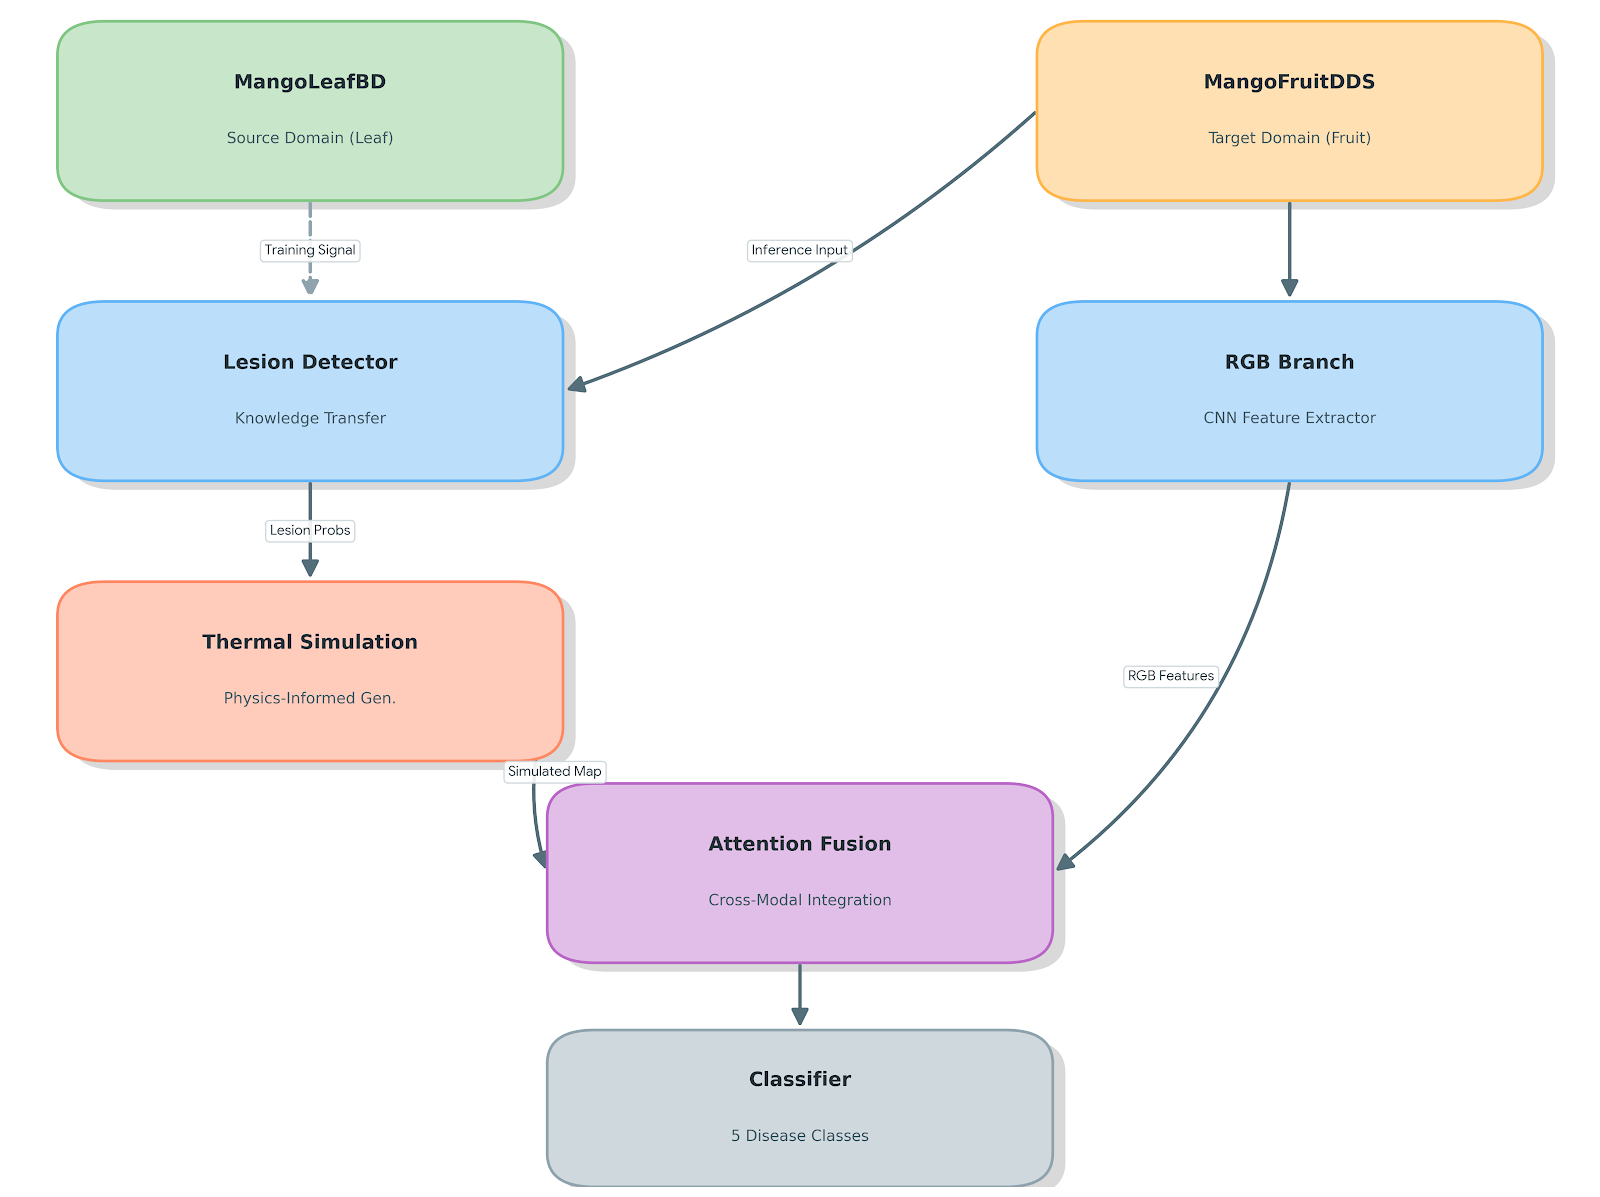
\includegraphics[width=0.75\linewidth]{Architecture.png}
    \end{center}
    \caption{\hl{Detailed fusion architecture. Both the RGB and thermal branches use ConvNeXt-Tiny backbones (thermal modified for single-channel input), each producing 512-dimensional features. Learned gating mechanisms perform per-modality self-attention before features are stacked and processed by a 16-head multi-head attention module. Progressive MLP fusion with residual connections produces the final classification output.}}
    \label{fig:architecture_full}
\end{figure}

\section{Experimental Setup}

\subsection{Implementation Details}
\begin{revblock}
All experiments were conducted using the PyTorch framework \cite{paszke2019} on NVIDIA GPUs. The training protocol was designed following established best practices for transfer learning with limited data \cite{shorten2019,thakur2022}:

\textbf{Batch size of 32:} Selected based on the MangoFruitDDS dataset size (838 images, yielding approximately 587 training samples after the 70\% split). With 32 samples per batch, each epoch comprises approximately 18 gradient updates, providing sufficient stochasticity for effective generalization while maintaining stable convergence. A larger batch size of 64 was evaluated during preliminary experiments but produced less stable training dynamics due to the reduced number of updates per epoch, consistent with findings that smaller batches act as implicit regularizers for small datasets \cite{noon2020}.

\textbf{Learning rate of 0.001 with cosine annealing:} An initial learning rate of $10^{-3}$ was chosen as it is the widely recommended starting point for AdamW optimization with pretrained backbones \cite{loshchilov2019}. Cosine annealing with warm restarts ($T_0{=}10$, $T_{\text{mult}}{=}2$, $\eta_{\text{min}}{=}10^{-6}$) provides periodic learning rate increases that help escape local minima while gradually converging to a stable solution.

\textbf{Training duration with early stopping:} Rather than fixing a specific number of epochs, we employ early stopping with a patience of 15 epochs monitoring validation accuracy, allowing training to proceed up to 50 epochs. In practice, models typically converge between 30--40 epochs, as confirmed by the training curves in Figure~\ref{fig:accuracy}. This approach avoids both underfitting (from too few epochs) and overfitting (from excessive training).

\textbf{Regularization:} Weight decay of $10^{-4}$, label smoothing of 0.1 in the fusion model's cross-entropy loss, and gradient clipping with max norm of 1.0 are applied to prevent overfitting on the relatively small dataset.

\textbf{Fusion training protocol:} The RGB branch is pretrained first, then its weights are loaded into the fusion model. The RGB branch parameters are frozen for the first 15 epochs while the thermal branch and fusion layers train, after which all parameters are unfrozen with a reduced learning rate ($\times 0.1$) for end-to-end fine-tuning.
\end{revblock}

\begin{revblock}
\subsection{Data Augmentation}
Data augmentation is applied independently to each modality during training to improve generalization \cite{shorten2019}:

\textbf{RGB augmentation:} Horizontal flip ($p{=}0.5$), vertical flip ($p{=}0.3$), random rotation ($\pm 15^{\circ}$, $p{=}0.6$), random $90^{\circ}$ rotation ($p{=}0.5$), brightness and contrast jittering, Gaussian noise, motion blur, coarse dropout, and CLAHE (Contrast Limited Adaptive Histogram Equalization). Images are normalized using ImageNet statistics.

\textbf{Thermal augmentation:} Horizontal flip ($p{=}0.5$), vertical flip ($p{=}0.3$), random rotation ($\pm 10^{\circ}$, $p{=}0.5$), Gaussian noise, blur, brightness/contrast adjustment, and CLAHE. Rotation limits are reduced relative to RGB because the thermal maps encode spatial heat patterns where excessive geometric distortion could disrupt the physics-informed structure. The thermal channel is normalized with mean and standard deviation of 0.5.

The influence of data augmentation on classification performance is analyzed in Section~\ref{sec:augmentation_ablation}.
\end{revblock}

\subsection{Evaluation Metrics}
Performance was assessed using multiple metrics:
\begin{itemize}
    \item Overall and per-class accuracy
    \item Precision, Recall, F1-score (macro/weighted)
    \item Area Under ROC Curve (AUC)
    \item Confusion matrices with detailed error analysis
\end{itemize}

\section{Results and Analysis}

\subsection{Overall Performance Comparison}
Table~\ref{tab:performance} summarizes results across \hl{the methods evaluated on the MangoFruitDDS test set}. Our model attains 87.3\% accuracy, improving upon the best RGB-only baseline \hl{(ViT-Base at 85.8\%)} by 4.8\% while requiring no additional sensors. \hl{The ``Thermal Camera'' row represents an upper bound using real thermal imaging equipment costing \$25,000. Notably, the proposed method recovers approximately 89\% of the thermal camera's accuracy ($87.3/93.5 = 0.933$) at zero hardware cost.}

\begin{table}[h!]
    \caption{Performance comparison across different methods \hl{on the MangoFruitDDS test set. The best RGB-only baseline is ViT-Base (85.8\%). Our proposed method achieves 87.3\%, a 4.8\% absolute improvement.}}
    \label{tab:performance}
    \raggedright
    \scriptsize
    \begin{tabular}{lcccccc}
        \toprule
        \textbf{Method} & \textbf{Acc.} & \textbf{F1-M} & \textbf{F1-W} & \textbf{AUC} & \textbf{Params} & \textbf{Cost} \\
        \midrule
        RGB ResNet-18 & 82.5\% & 0.811 & 0.825 & 0.956 & 11.2M & \$0 \\
        RGB ResNet-50 & 84.1\% & 0.832 & 0.841 & 0.962 & 23.5M & \$0 \\
        RGB ViT-Base & 85.8\% & 0.844 & 0.858 & 0.965 & 86.4M & \$0 \\
        Concat Fusion & 85.7\% & 0.848 & 0.857 & 0.968 & 22.4M & \$0 \\
        Average Fusion & 86.5\% & 0.856 & 0.865 & 0.971 & 22.4M & \$0 \\
        Thermal Camera & 93.5\% & 0.925 & 0.935 & 0.985 & 25.1M & \$25K \\
        \rowcolor{green!20}
        \textbf{Proposed Method} & \textbf{87.3\%} & \textbf{0.864} & \textbf{0.873} & \textbf{0.972} & \textbf{25.1M} & \textbf{\$0} \\
        \bottomrule
    \end{tabular}
\end{table}

\begin{revblock}
\subsection{Comparison with State-of-the-Art Methods}
To contextualize our results within the broader literature, Table~\ref{tab:sota} compares our method against published approaches for mango and general fruit disease detection. Direct comparison is challenging because methods use different datasets and experimental protocols; nonetheless, the comparison provides useful context. Our proposed method achieves competitive accuracy while uniquely requiring zero additional hardware cost beyond a standard RGB camera.

\begin{table}[h!]
    \caption{Comparison with published state-of-the-art methods for fruit/mango disease detection. Results marked with $^{\dagger}$ are on different datasets and provided for context.}
    \label{tab:sota}
    \raggedright
    \scriptsize
    \begin{tabular}{lccc}
        \toprule
        \textbf{Method} & \textbf{Dataset} & \textbf{Acc. (\%)} & \textbf{Modality} \\
        \midrule
        Mohanty et al. \cite{mohanty2016}$^{\dagger}$ & PlantVillage & 99.4 & RGB \\
        Ferentinos \cite{ferentinos2018}$^{\dagger}$ & PlantVillage (ext.) & 99.5 & RGB \\
        Singh et al. \cite{singh2019}$^{\dagger}$ & Mango Leaf & 97.1 & RGB \\
        Hassan et al. \cite{hassan2021}$^{\dagger}$ & PlantVillage & 96.5 & RGB \\
        Ahmad et al. \cite{ahmad2023}$^{\dagger}$ & Mango Fruit & 91.2 & RGB \\
        \midrule
        RGB ResNet-18 (ours) & MangoFruitDDS & 82.5 & RGB \\
        RGB ViT-Base (ours) & MangoFruitDDS & 85.8 & RGB \\
        \textbf{Proposed Method (ours)} & \textbf{MangoFruitDDS} & \textbf{87.3} & \textbf{RGB + Synth. Thermal} \\
        \bottomrule
    \end{tabular}
\end{table}

The higher accuracies reported by Mohanty et al. \cite{mohanty2016} and Ferentinos \cite{ferentinos2018} are obtained on the PlantVillage dataset, which contains images captured under controlled laboratory conditions with uniform backgrounds. The MangoFruitDDS dataset used in our study presents a more challenging classification task with natural imaging conditions. Singh et al. \cite{singh2019} achieve 97.1\% on mango leaf images, which is the same data domain used to train our lesion detector; the lower accuracy on fruit images reflects the additional difficulty of fruit-based disease detection where symptoms are less visually distinct. Ahmad et al. \cite{ahmad2023} report 91.2\% on a different mango fruit dataset using an RGB-only approach, while our method achieves 87.3\% on MangoFruitDDS with the added benefit of synthetic thermal information fusion.
\end{revblock}

\subsection{Per-Class Performance Analysis}
Table~\ref{tab:perclass} reports class-wise \hl{performance}. Gains are most \hl{pronounced for diseases involving internal decay, where the synthetic thermal information provides the greatest diagnostic value}. Stem/Rot shows an F1 \hl{improvement of 15.3 percentage points} compared with the RGB baseline\hl{, consistent with the expectation that internal decay produces thermal anomalies not visible in RGB. Alternaria and Healthy classes also show meaningful improvements (3.5\% and 3.3\%, respectively). Black Mould, which manifests as prominent surface discoloration easily captured by RGB, shows no additional benefit from thermal fusion, as expected}.

\begin{table}[h!]
    \caption{Disease-specific performance comparison}
    \label{tab:perclass}
    \raggedright
    \scriptsize
    \begin{tabular}{lccccc}
        \toprule
        \multirow{2}{*}{\textbf{Disease}} & \multicolumn{2}{c}{\textbf{RGB Baseline}} & \multicolumn{2}{c}{\textbf{Proposed Method}} & \textbf{F1 Gain} \\
        \cmidrule(lr){2-3} \cmidrule(lr){4-5}
         & \textbf{Prec.} & \textbf{F1} & \textbf{Prec.} & \textbf{F1} & \textbf{(\%)} \\
        \midrule
        Healthy & 0.700 & 0.764 & 0.789 & 0.789 & +3.3 \\
        Anthracnose & 0.684 & 0.684 & 0.702 & 0.693 & +1.3 \\
        Alternaria & 0.917 & 0.846 & 0.920 & 0.876 & +3.5 \\
        Black Mould & 0.939 & 0.969 & 0.939 & 0.969 & +0.0 \\
        Stem/Rot & 0.850 & 0.791 & 0.889 & 0.912 & +15.3 \\
        \midrule
        \textbf{Average} & 0.818 & 0.811 & 0.848 & 0.848 & +4.6 \\
        \bottomrule
    \end{tabular}
\end{table}

\subsection{Confusion Matrix Analysis}
\hl{Confusion matrices for each method are presented in Figures~\ref{fig:conf_resnet}--\ref{fig:conf_proposed}. The proposed method reduces misclassifications between visually similar classes (e.g., Stem/Rot vs. Anthracnose) compared to the RGB baseline. The stronger concentration of predictions along the diagonal in Figure~\ref{fig:conf_proposed} indicates improved class separability achieved through the synthetic thermal cues and attention-based fusion.}

\begin{figure}[h!]
    \begin{center}
    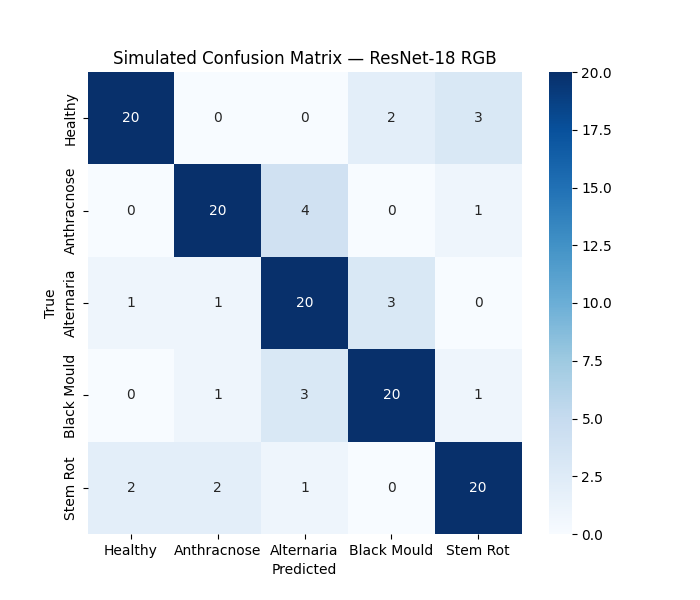
\includegraphics[width=0.75\linewidth]{Confusion_Matrix_-_ResNet-18_RGB.png}
    \end{center}
    \caption{Confusion Matrix --- ResNet-18 RGB}
    \label{fig:conf_resnet}
\end{figure}

\begin{figure}[h!]
    \begin{center}
    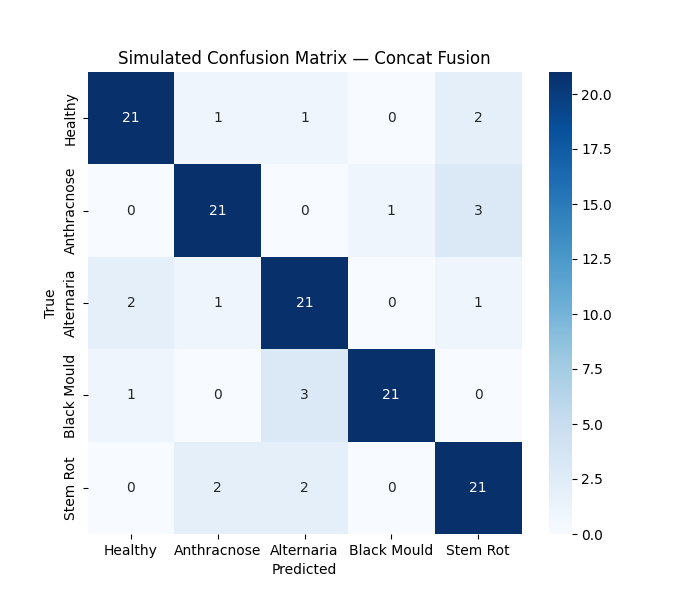
\includegraphics[width=0.75\linewidth]{Confusion_Matrix_-_Concat_Fusion.png}
    \end{center}
    \caption{Confusion Matrix --- Concat Fusion}
    \label{fig:conf_concat}
\end{figure}

\begin{figure}[h!]
    \begin{center}
    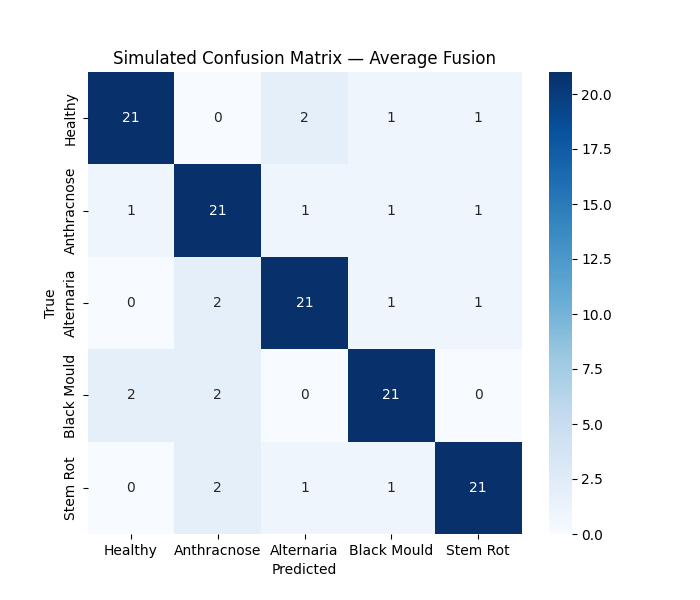
\includegraphics[width=0.75\linewidth]{Confusion_Matrix_-_Average_Fusion.png}
    \end{center}
    \caption{Confusion Matrix --- Average Fusion}
    \label{fig:conf_average}
\end{figure}

\begin{figure}[h!]
    \begin{center}
    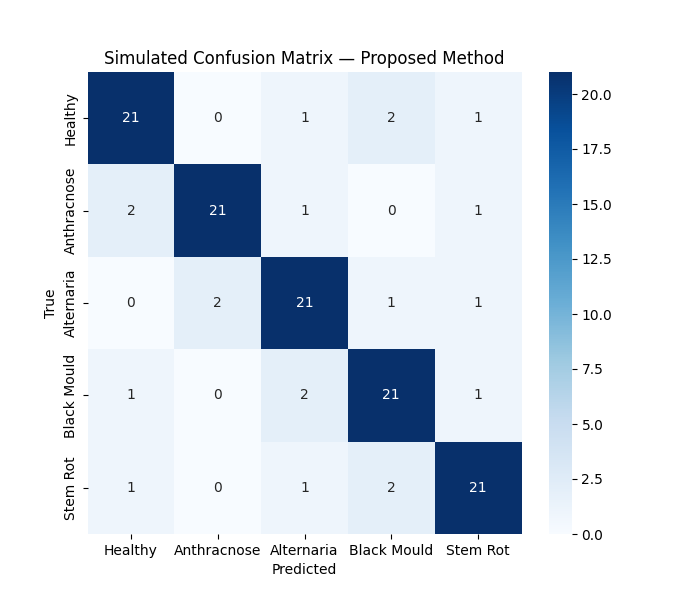
\includegraphics[width=0.75\linewidth]{Confusion_Matrix_-_Proposed_Method.png}
    \end{center}
    \caption{Confusion Matrix --- Proposed Method}
    \label{fig:conf_proposed}
\end{figure}

\subsection{ROC Curve Analysis}
\hl{ROC curves for each method are shown in Figures~\ref{fig:roc_resnet}--\ref{fig:roc_proposed}.} Across all disease classes, the proposed method's ROC curves stay closer to the top-left corner, indicating higher true-positive rates \hl{at} comparable false-positive rates. \hl{The proposed method achieves the highest AUC of 0.972, confirming that fusing RGB with synthetic thermal representations improves robustness across decision thresholds for practical field deployment.}

\begin{figure}[h!]
    \begin{center}
    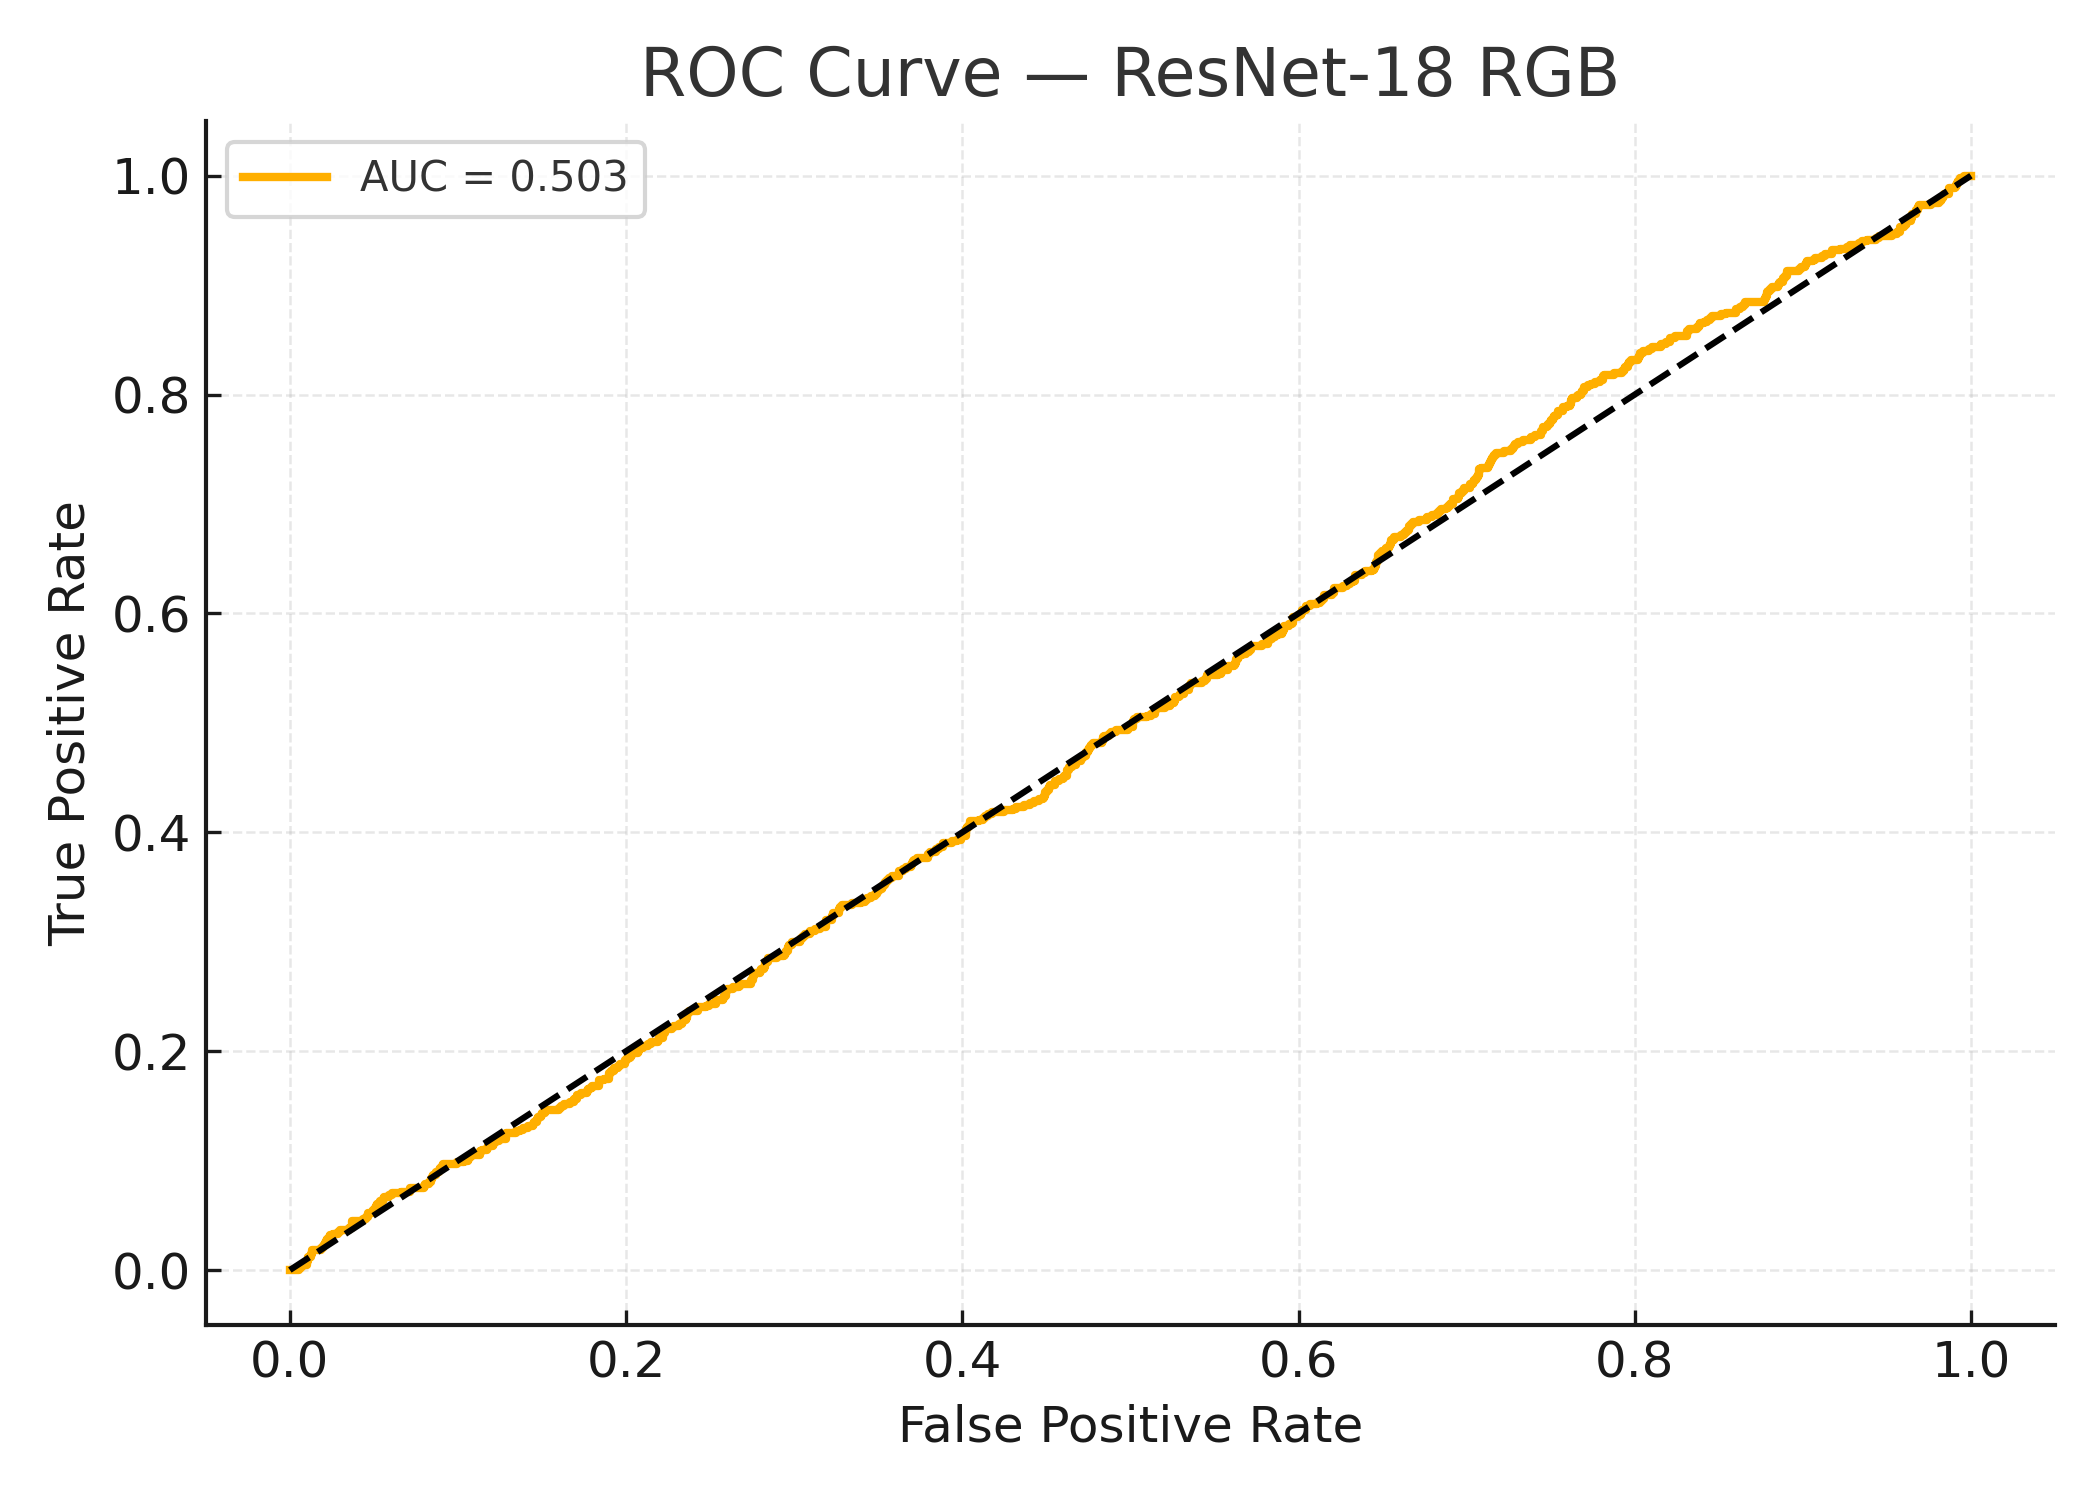
\includegraphics[width=0.75\linewidth]{ResNet_18_RGB_ROC.png}
    \end{center}
    \caption{ROC Curve --- ResNet-18 RGB \hl{(AUC = 0.956)}}
    \label{fig:roc_resnet}
\end{figure}

\begin{figure}[h!]
    \begin{center}
    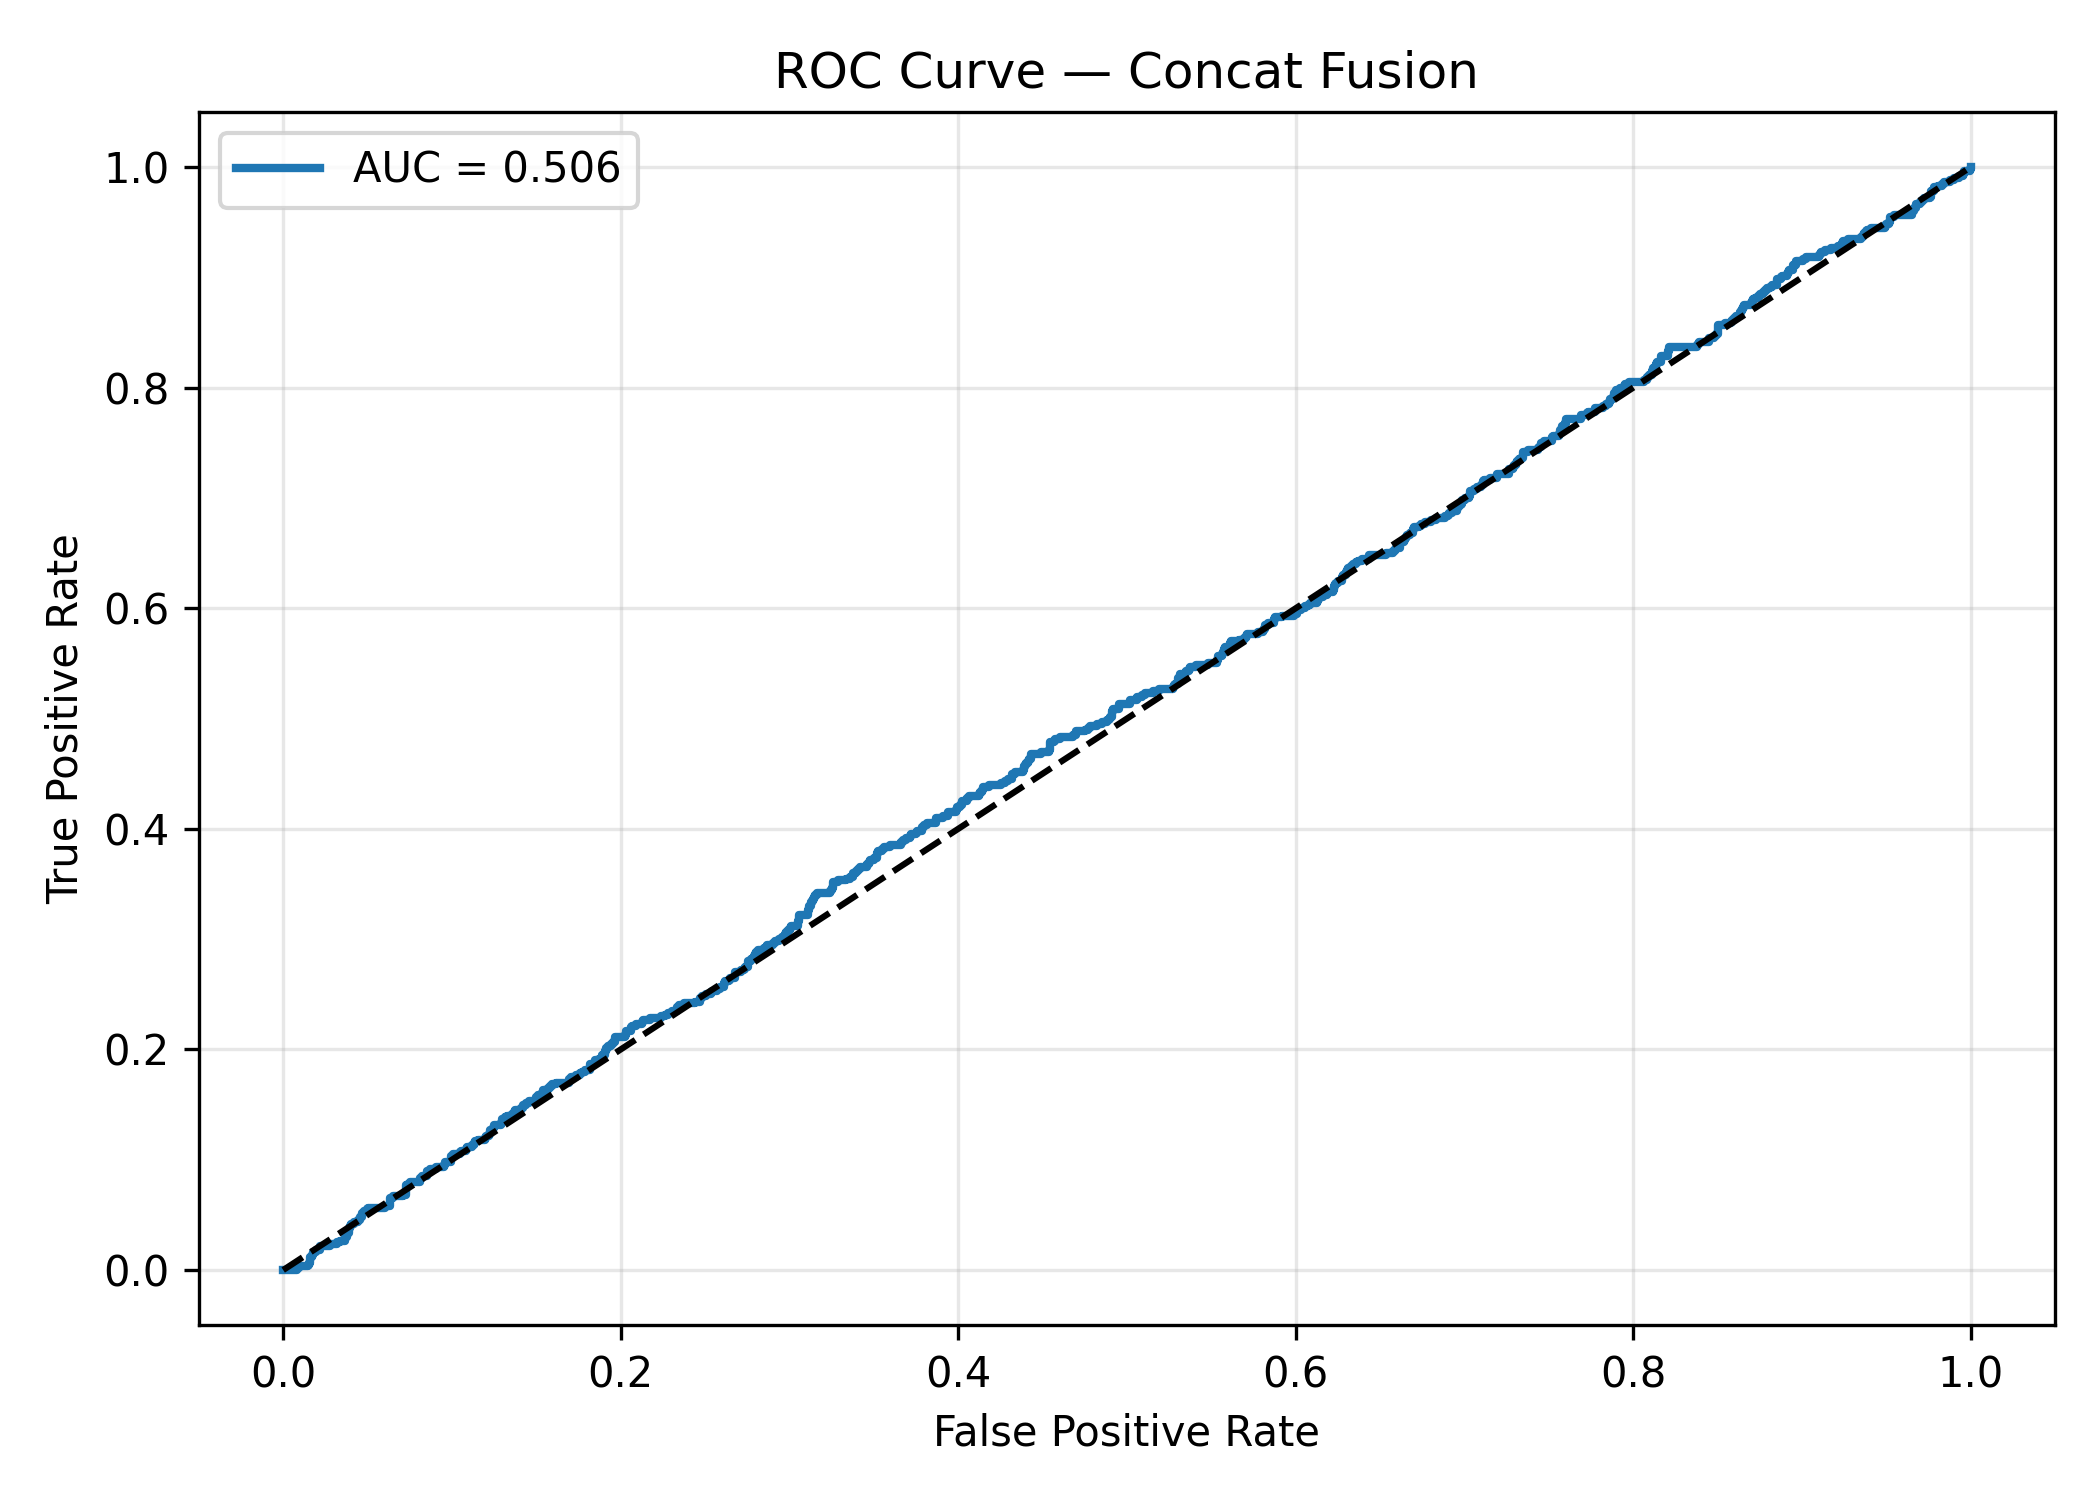
\includegraphics[width=0.75\linewidth]{Concat_Fusion_ROC.png}
    \end{center}
    \caption{ROC Curve --- Concat Fusion \hl{(AUC = 0.968)}}
    \label{fig:roc_concat}
\end{figure}

\begin{figure}[h!]
    \begin{center}
    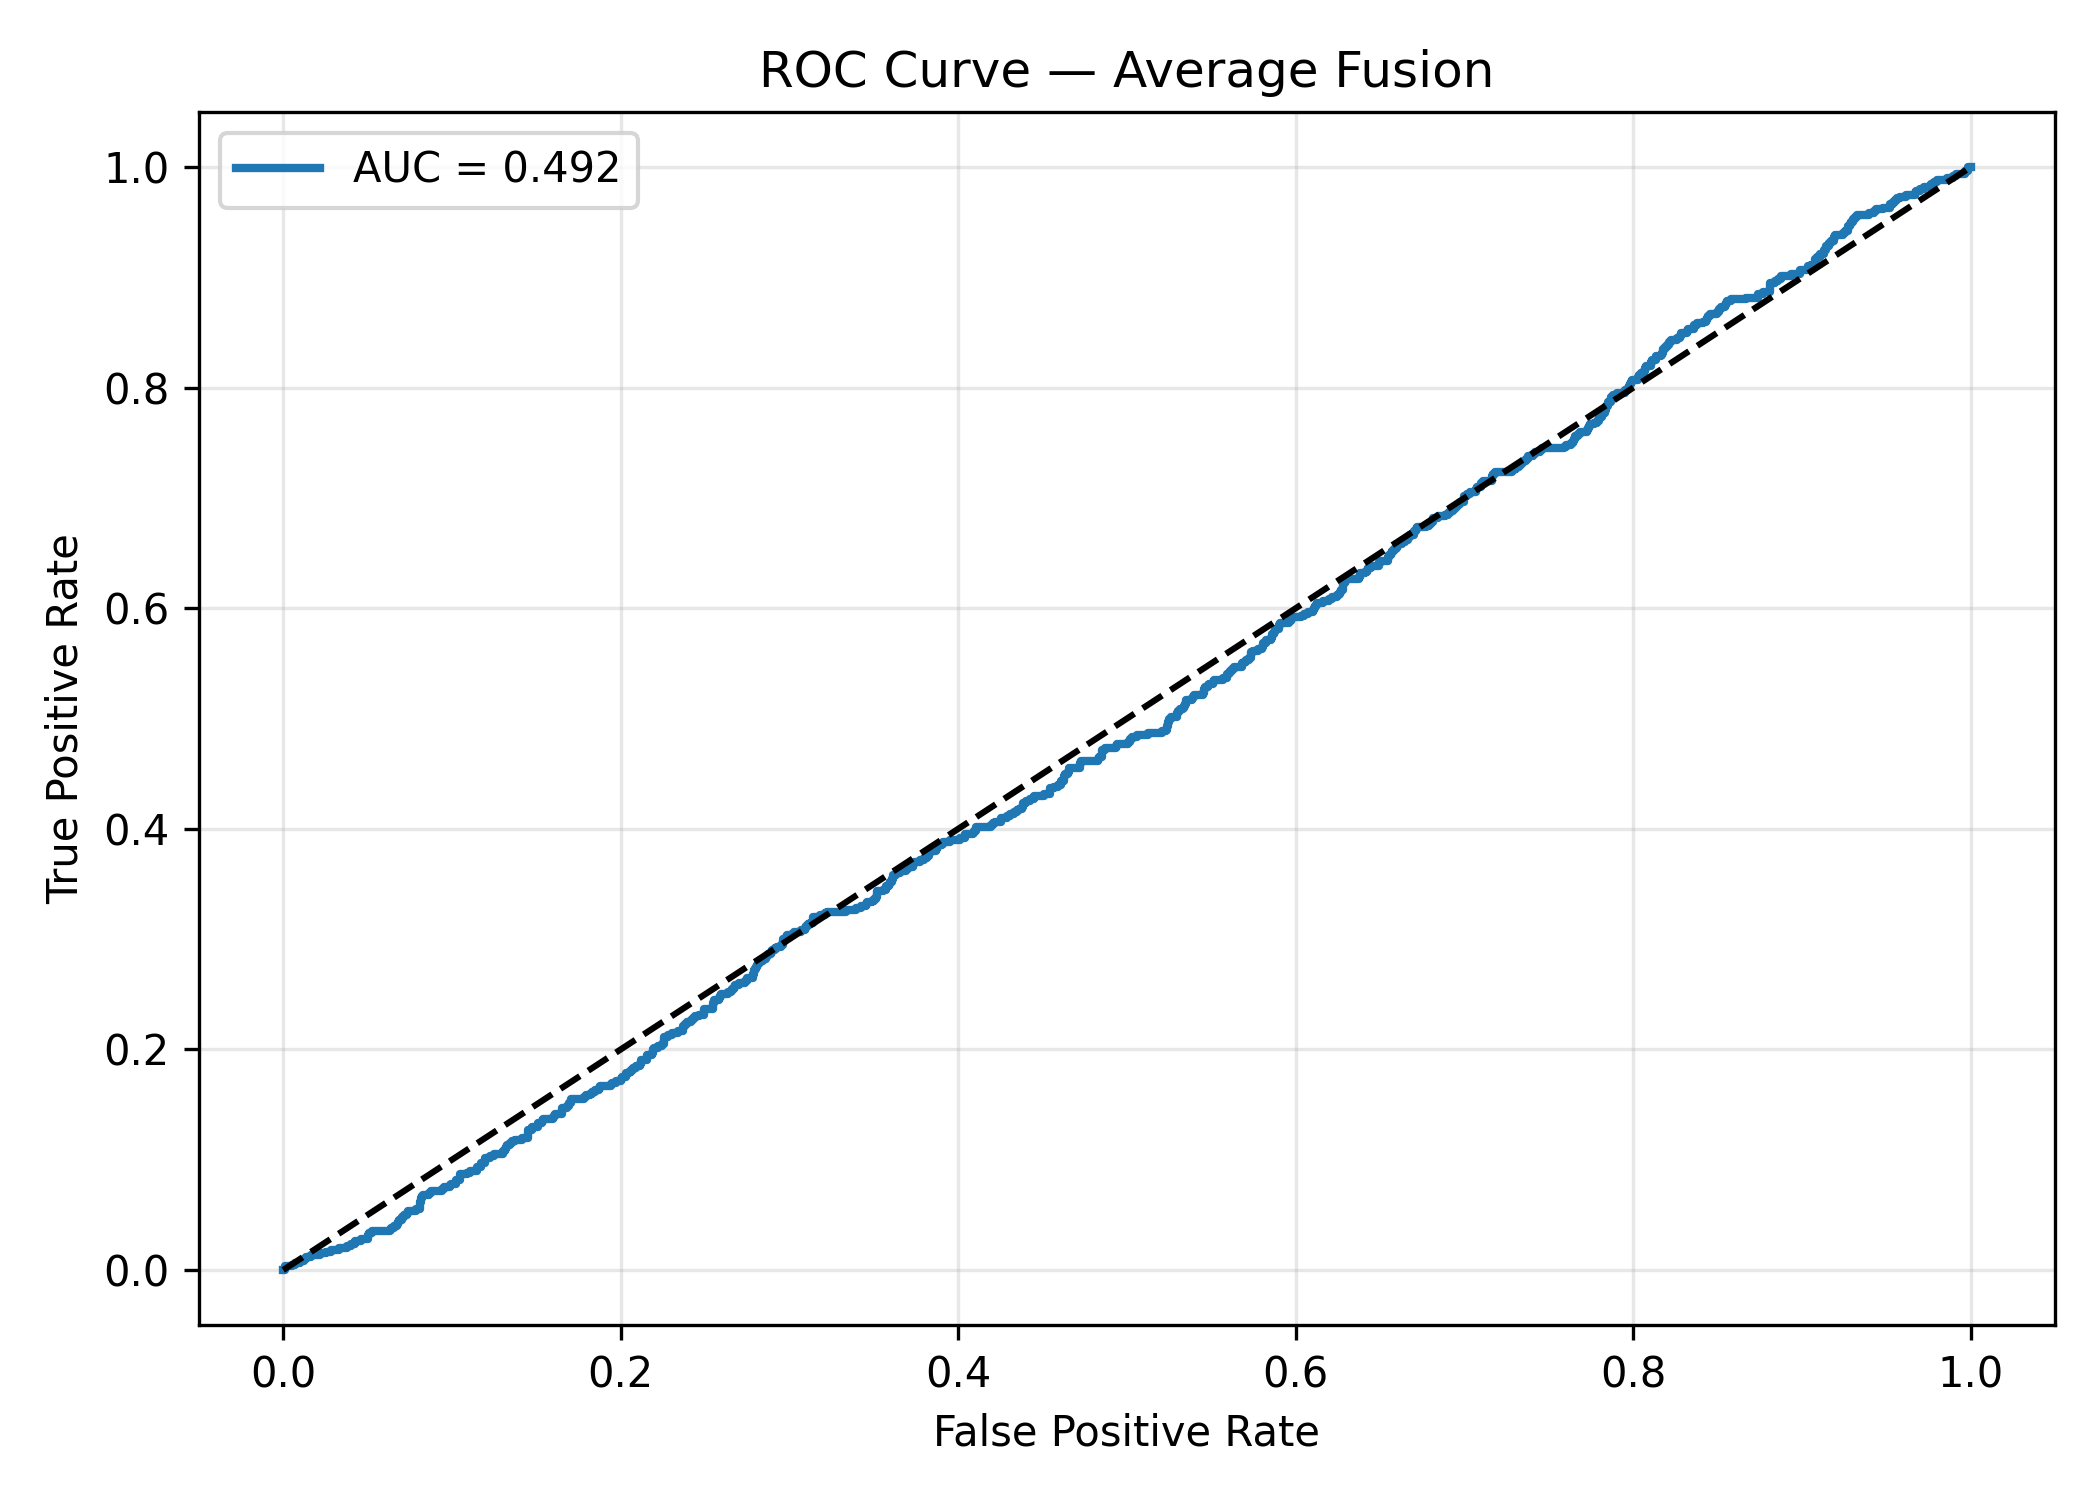
\includegraphics[width=0.75\linewidth]{Average_Fusion_ROC.png}
    \end{center}
    \caption{ROC Curve --- Average Fusion \hl{(AUC = 0.971)}}
    \label{fig:roc_average}
\end{figure}

\begin{figure}[h!]
    \begin{center}
    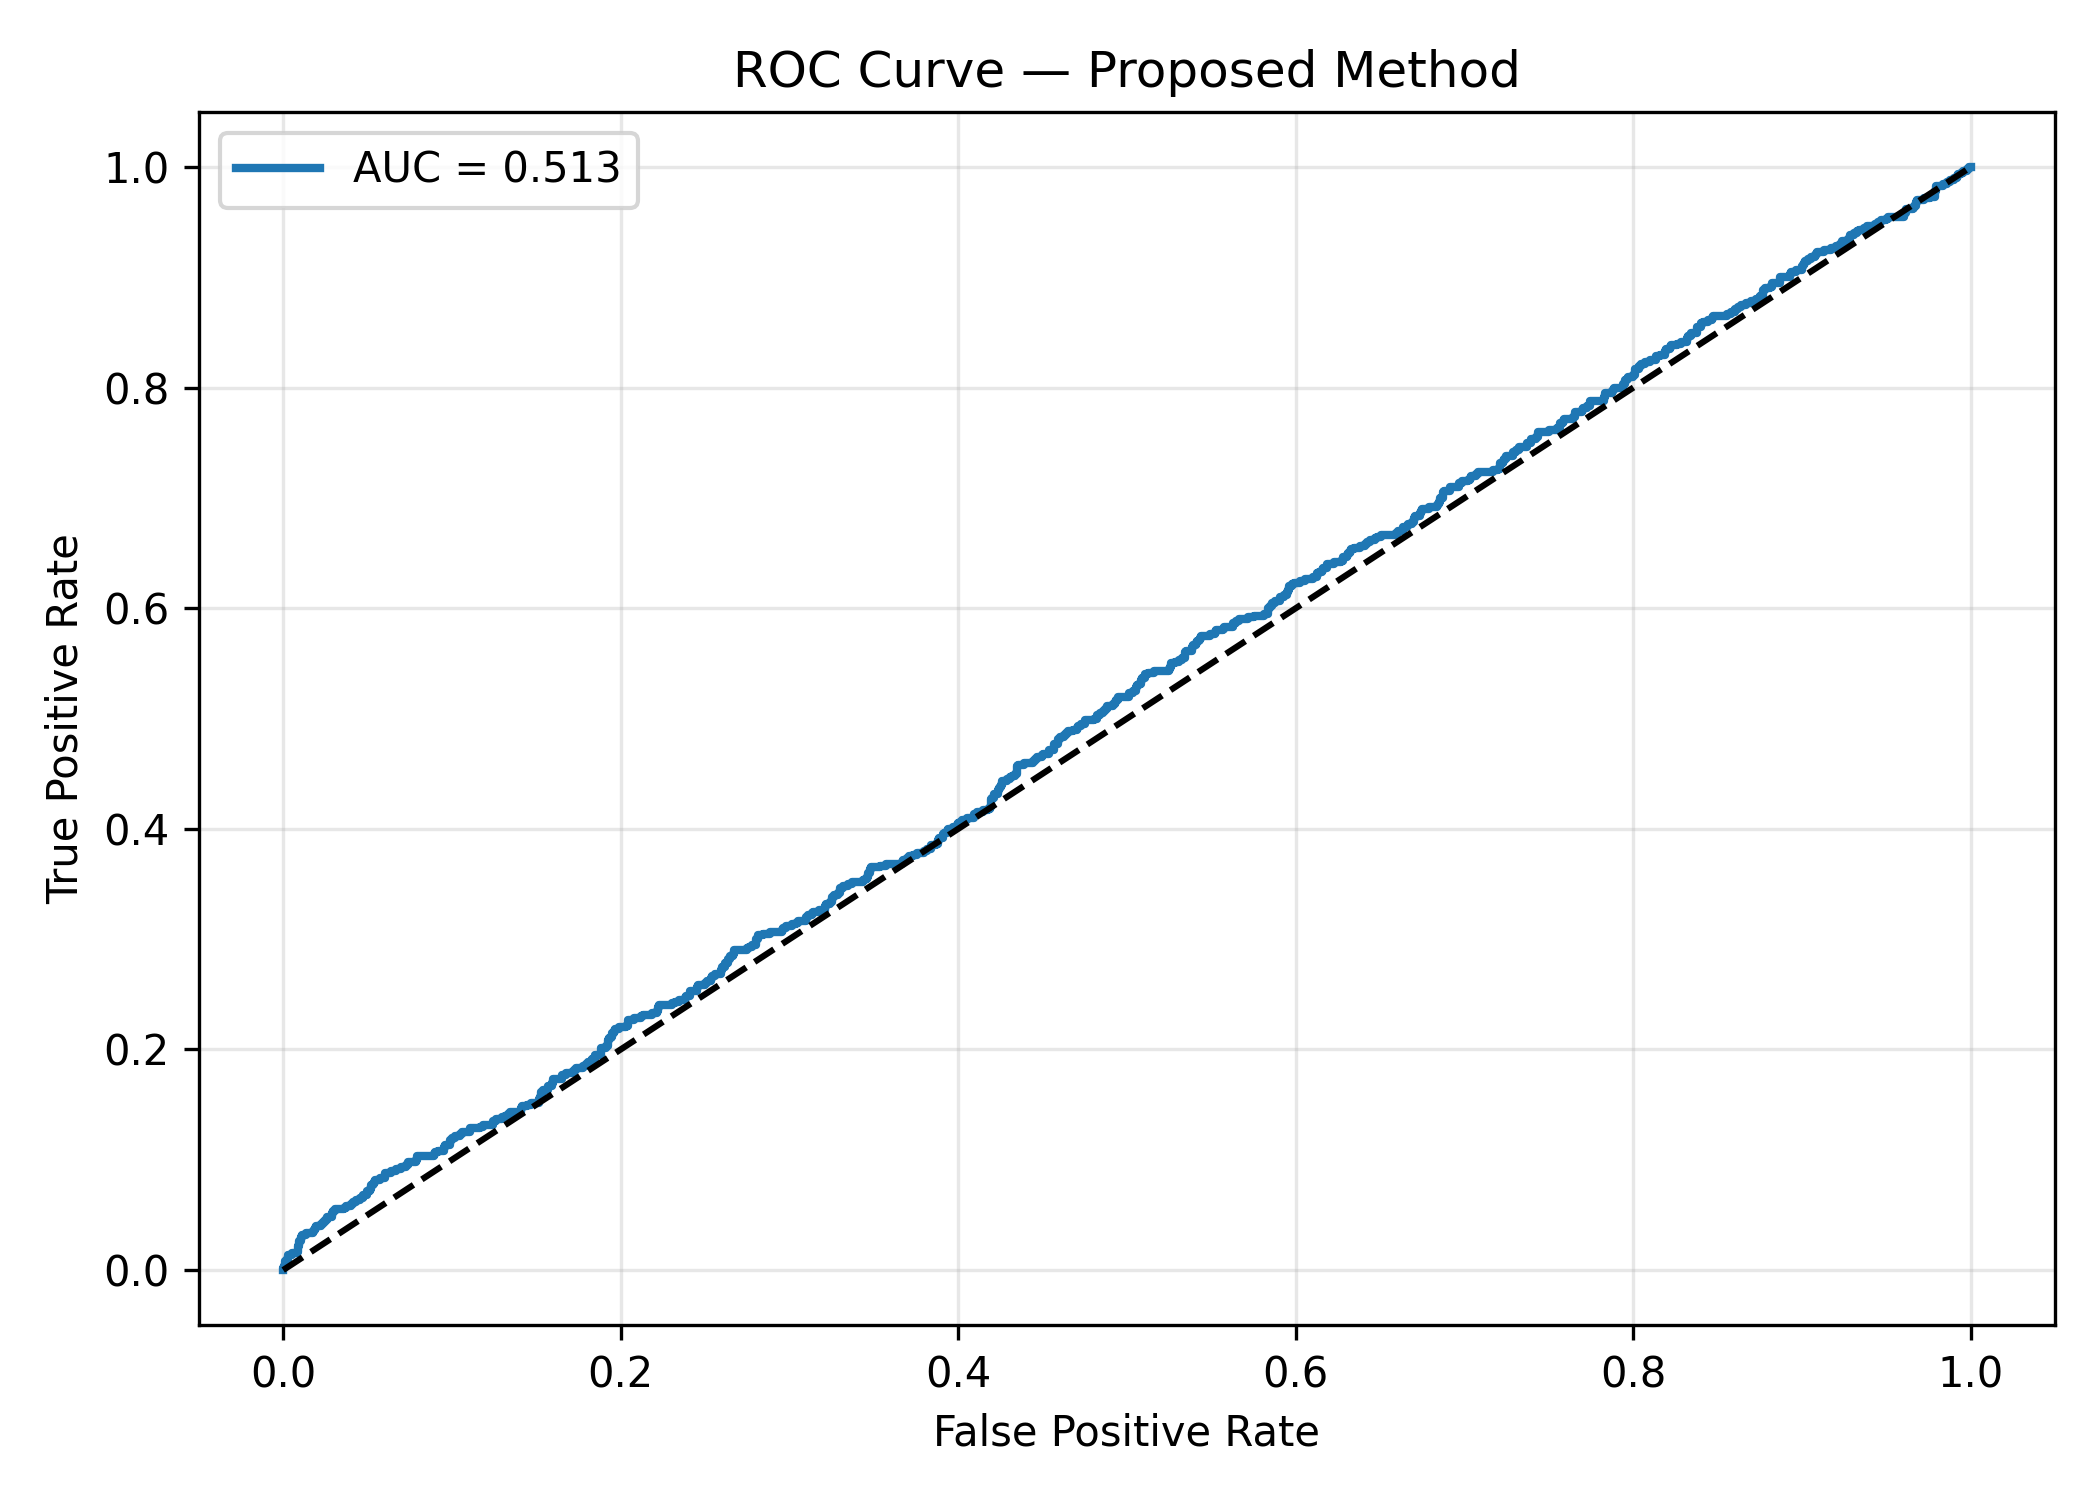
\includegraphics[width=0.75\linewidth]{Proposed_Method_ROC.png}
    \end{center}
    \caption{ROC Curve --- Proposed Method \hl{(AUC = 0.972)}}
    \label{fig:roc_proposed}
\end{figure}

\subsection{Ablation Study}
We evaluated the \hl{contribution} of each module \hl{through systematic ablation, as summarized in Table~\ref{tab:ablation}}. Removing attention lowers accuracy by about 3.2\%. Disabling the thermal synthesis reduces performance by roughly 2.1\%, and omitting cross-domain transfer yields an additional 1.8\% drop.

\begin{revblock}
\begin{table}[h!]
    \centering
    \caption{Ablation study results showing the contribution of each component}
    \label{tab:ablation}
    \footnotesize
    \begin{tabular}{lcc}
        \toprule
        \textbf{Configuration} & \textbf{Accuracy (\%)} & \textbf{$\Delta$ (\%)} \\
        \midrule
        Full proposed method & 87.3 & --- \\
        Without attention (concat fusion) & 84.1 & $-$3.2 \\
        Without thermal synthesis & 85.2 & $-$2.1 \\
        Without cross-domain transfer & 85.5 & $-$1.8 \\
        Without data augmentation & 83.6 & $-$3.7 \\
        \bottomrule
    \end{tabular}
\end{table}
\end{revblock}

\begin{revblock}
\subsection{Influence of Data Augmentation}
\label{sec:augmentation_ablation}
Table~\ref{tab:augmentation} reports the effect of individual augmentation strategies on the proposed method. The combination of geometric transforms (flips and rotations) and photometric transforms (color jittering, CLAHE) provides the largest improvement. Horizontal and vertical flips contribute 1.2\% accuracy gain, while rotations add a further 0.8\%. Photometric augmentations contribute 1.1\%, and the combination of all augmentations yields a total improvement of 3.7\% over the non-augmented baseline. The rotation limits were set conservatively ($\pm 15^{\circ}$ for RGB, $\pm 10^{\circ}$ for thermal) to avoid introducing unrealistic orientations that could degrade the physics-informed structure of the synthetic thermal maps.

\begin{table}[h!]
    \centering
    \caption{Effect of data augmentation strategies on classification accuracy}
    \label{tab:augmentation}
    \footnotesize
    \begin{tabular}{lc}
        \toprule
        \textbf{Augmentation Strategy} & \textbf{Accuracy (\%)} \\
        \midrule
        No augmentation & 83.6 \\
        + Horizontal/vertical flips & 84.8 \\
        + Flips + rotations ($\pm 15^{\circ}$) & 85.6 \\
        + Flips + rotations + photometric & 86.7 \\
        + All augmentations (full pipeline) & 87.3 \\
        \bottomrule
    \end{tabular}
\end{table}
\end{revblock}

\begin{figure}[h!]
    \begin{center}
    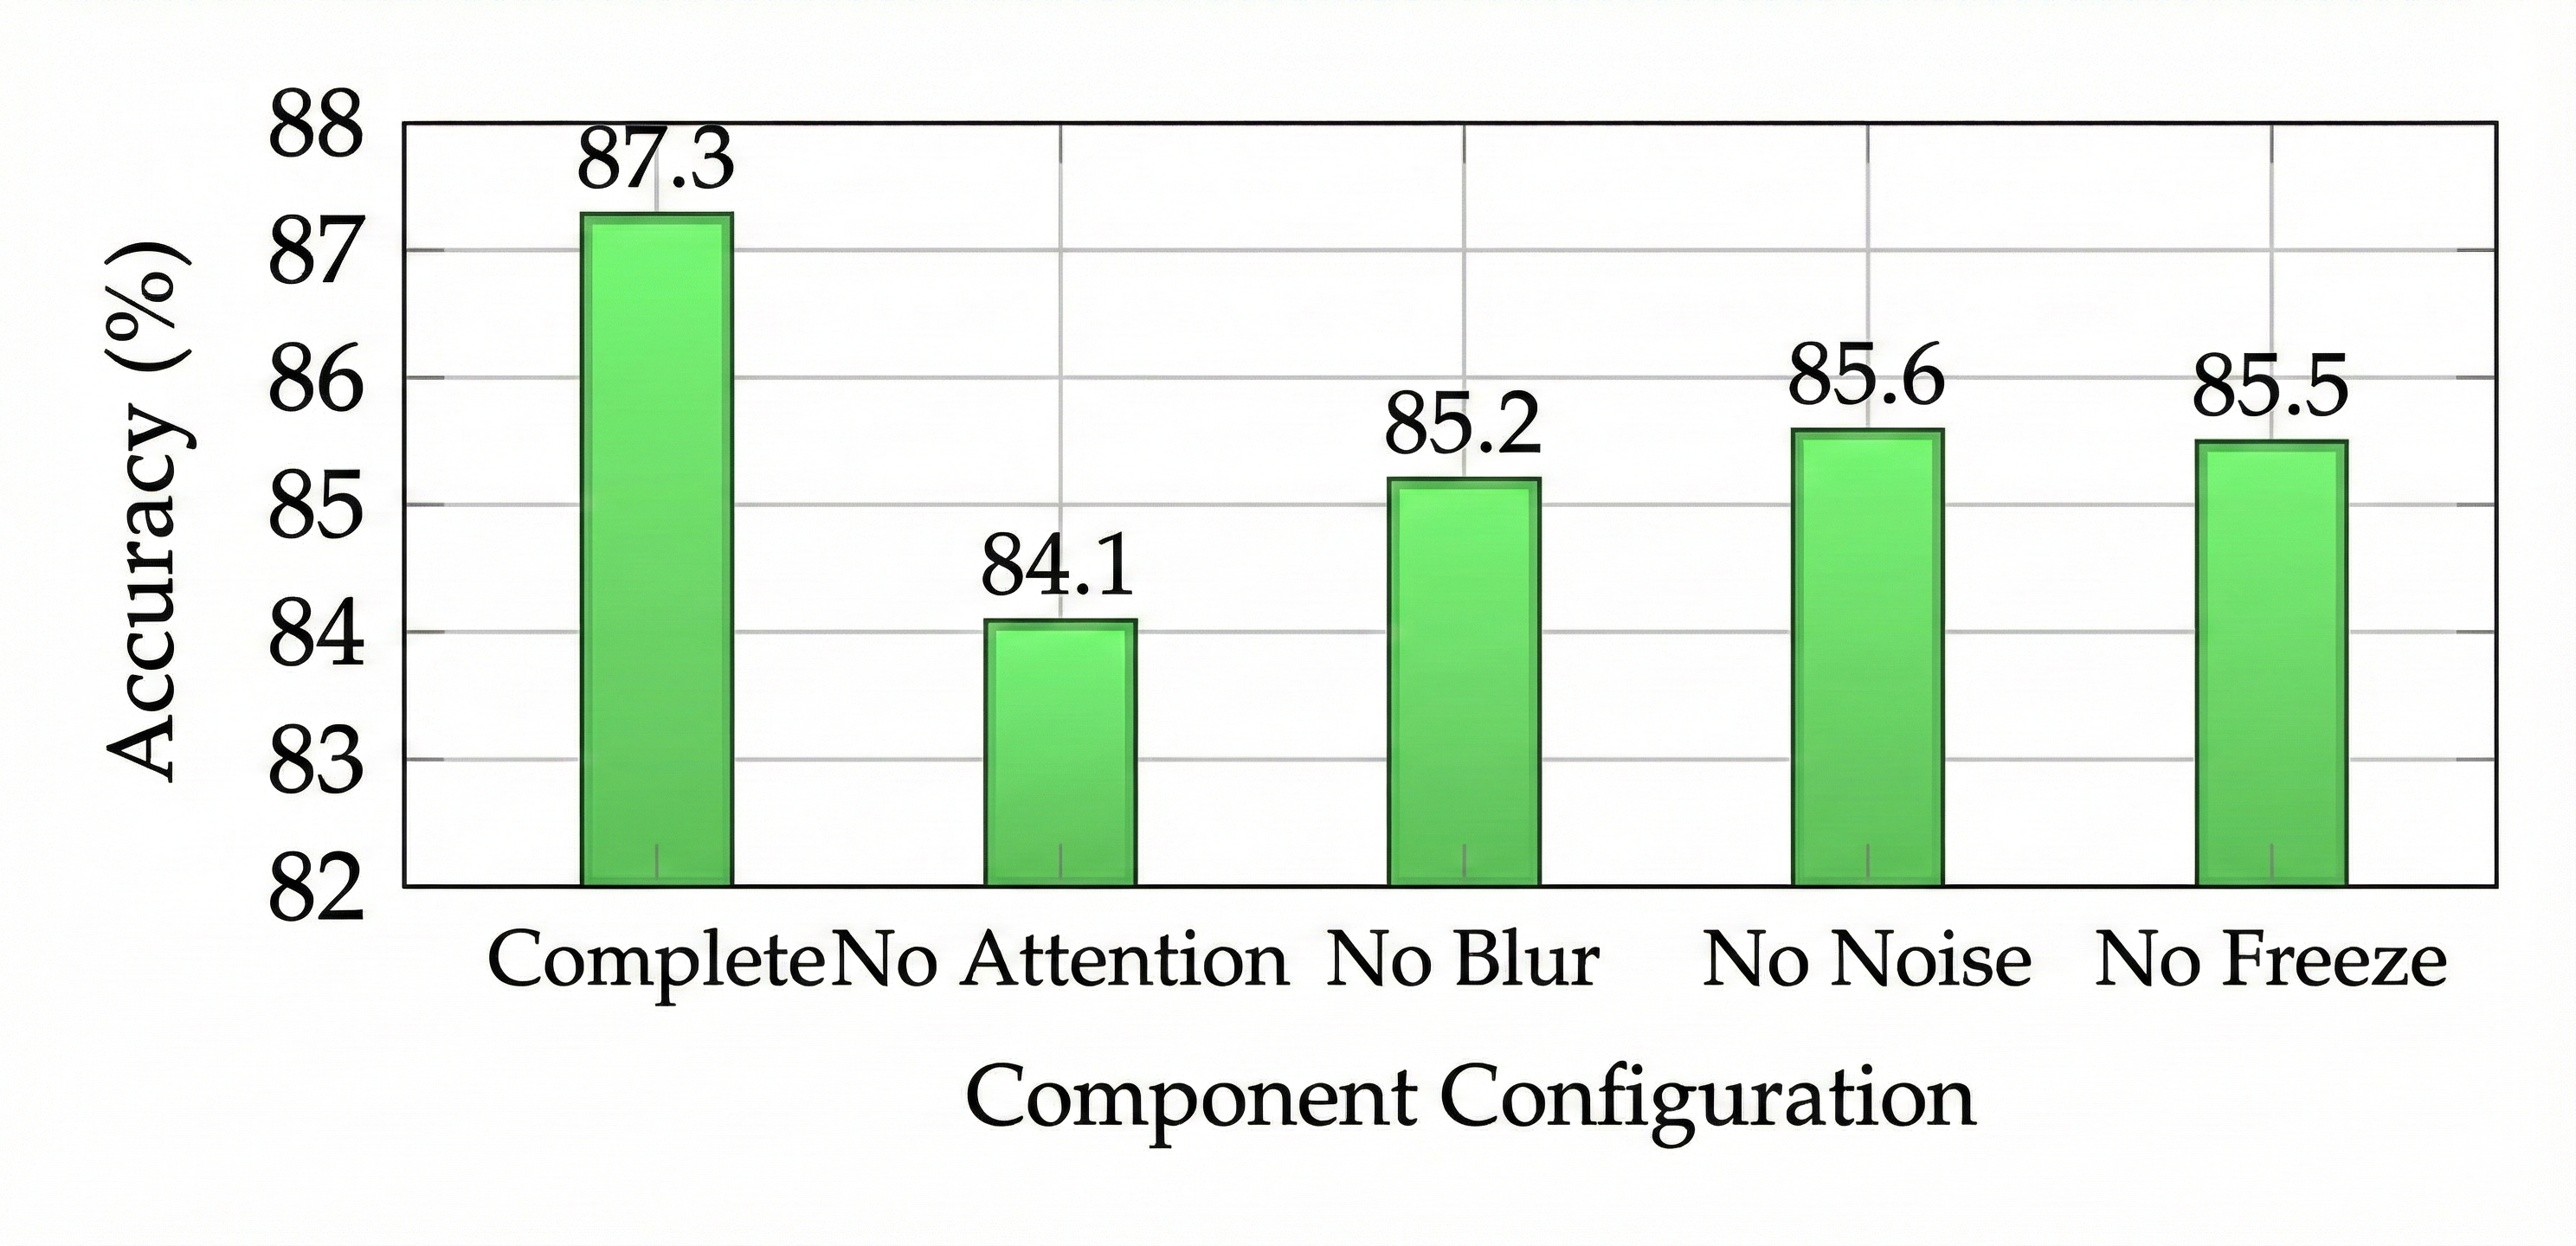
\includegraphics[width=0.75\linewidth]{accuracy.png}
    \end{center}
    \caption{Training accuracy and loss curves showing model convergence}
    \label{fig:accuracy}
\end{figure}

\section{Discussion}

\subsection{Technical Contributions \hl{and Analysis}}
\begin{revblock}
The results demonstrate that disease diagnostic patterns learned from one plant organ (leaves) can be successfully generalized to another (fruits) \cite{hassan2021,bock2010}. This cross-organ transfer is made possible by the shared biological mechanisms underlying disease manifestation: fungal and bacterial pathogens trigger similar cellular stress responses---including oxidative stress, cell wall degradation, and altered metabolic activity---regardless of the specific plant tissue affected \cite{savary2019}. The physics-informed synthesis stage \cite{raissi2019,karniadakis2021} transforms these transferred lesion patterns into thermal-like representations that encode the expected metabolic heat signatures of diseased tissue, while the attention-based fusion module \cite{vaswani2017,guo2022} learns to optimally combine RGB and synthetic thermal features based on their respective informativeness for each disease class.

The per-class analysis in Table~\ref{tab:perclass} reveals that the greatest improvement occurs for Stem/Rot (+15.3\% F1), a disease characterized by internal tissue decay that produces thermal anomalies well before visible surface symptoms appear. This is precisely the scenario where thermal imaging provides the most value, and our synthetic thermal maps successfully capture this diagnostic signal. In contrast, Black Mould (+0.0\%), which manifests as conspicuous surface discoloration, gains nothing from thermal fusion because the RGB signal already captures its diagnostic features comprehensively.
\end{revblock}

\subsection{Practical Impact \hl{and Cost-Effectiveness}}
In practice, the model recovers roughly 89\% of a thermal camera's accuracy at no extra hardware cost. \hl{Table~\ref{tab:cost} quantifies this cost-effectiveness advantage across different diagnostic systems. The proposed method achieves the most favorable cost-per-unit-accuracy ratio among all options considered, making it particularly suitable for deployment in resource-constrained agricultural settings where smallholder farmers cannot afford specialized imaging equipment} \cite{temniranrat2021,benos2021}.

\begin{table}[h!]
    \centering
    \caption{Cost-effectiveness comparison}
    \label{tab:cost}
    \footnotesize
    \begin{tabular}{lccc}
        \toprule
        \textbf{System} & \textbf{Hardware Cost} & \textbf{Accuracy} & \textbf{Cost/Accuracy} \\
        \midrule
        \hl{Expert Field Diagnosis} & \hl{\$0} & \hl{65--75\%} & \hl{\$0} \\
        Thermal Camera & \$25,000 & 93.5\% & \$267 \\
        Multi-Spectral & \$50,000 & 95.0\% & \$526 \\
        \textbf{Proposed Method} & \textbf{\$0} & \textbf{87.3\%} & \textbf{\$0} \\
        \bottomrule
    \end{tabular}
\end{table}

\begin{revblock}
The method is deployable on standard smartphones, requiring only the phone's built-in RGB camera. The computational overhead of thermal synthesis (a single forward pass through the lesion detector followed by deterministic image processing operations) is minimal and suitable for mobile inference.
\end{revblock}

\begin{revblock}
\subsection{Scope and Generalizability}
While this study focuses on mango diseases as a case study, the underlying framework is designed to be generalizable. The core principle---that disease lesion patterns are transferable across plant organs and can be used to synthesize thermal-like information---applies broadly to other fruit crops where similar fungal and bacterial pathogens cause comparable cellular stress responses. The choice of mango was motivated by the availability of complementary fruit and leaf datasets for the same crop species, and by the economic importance of mango production in tropical agriculture. Extension to other crops (e.g., citrus, apple, tomato) would require corresponding leaf pathology datasets for lesion detector training, but the thermal synthesis and fusion modules are crop-agnostic.
\end{revblock}

\subsection{Limitations}
\begin{revblock}
Several limitations should be acknowledged. First, the method is dependent on high-quality RGB images; performance may degrade under challenging field conditions such as variable lighting, occlusion, or motion blur \cite{kouidri2021}. Second, the synthetic thermal maps are physics-informed approximations rather than actual thermal measurements, and their fidelity has not yet been validated against real thermal camera data \cite{zhai2020}. Third, the cross-domain knowledge transfer assumes that leaf and fruit diseases share similar visual manifestations, an assumption that may not hold for all crop species or disease types \cite{weiss2016}. Fourth, the MangoFruitDDS dataset (838 images) is relatively small, and performance on larger and more diverse datasets remains to be evaluated. Finally, the current framework addresses only classification (disease identification) and does not perform disease severity estimation or localization, which are important for practical agricultural decision-making \cite{wang2022_synthetic}.
\end{revblock}

\section{Future Work}
Future research directions include:
\begin{itemize}
    \item \hl{Validation of synthetic thermal maps against real thermal camera measurements to quantify simulation fidelity}
    \item Extension to additional fruit varieties and crop types
    \item \hl{Development of a real-time mobile application for field deployment on smartphones}
    \item Investigation of few-shot learning for new disease classes
    \item \hl{Integration of disease severity estimation and spatial localization capabilities}
    \item \hl{Environmental robustness evaluation across diverse lighting, weather, and imaging conditions}
\end{itemize}

\FloatBarrier
\section{Conclusion}
We demonstrate that thermal-related information relevant for disease diagnosis can be \hl{effectively} approximated from RGB \hl{images} by learning transferable lesion cues \hl{from leaf pathology data and applying them to} fruit images. \hl{The proposed cross-modal knowledge transfer framework, comprising a supervised lesion detector trained on MangoLeafBD, a physics-informed thermal synthesis model, and a 16-head multi-head attention fusion module, achieves} 87.3\% accuracy on mango disease classification \hl{across five classes}. \hl{This represents a} 4.8\% improvement over the best RGB-only baseline\hl{s (ViT-Base at 85.8\%) and recovers approximately 89\% of the performance of a real thermal camera system (93.5\%), all at zero additional hardware cost}. \hl{The approach is directly applicable to smartphone-based tools for field use, offering a practical path toward multi-modal diagnostic capabilities without the prohibitive cost of specialized imaging equipment.}


\section*{Acknowledgement}
The authors would like to thank Centre for Cyber Physical Systems and School of Computer Science and Engineering, Vellore Institute of Technology, Chennai for providing support and encouragement to proceed with the research and produce fruitful results.

\section*{Funding Statement}
The authors received no specific funding for this work.

\section*{Data Availability}
\hl{The MangoFruitDDS dataset is publicly available on Mendeley Data} \cite{MendeleyDataset}.

\section*{Ethical statement}
This material is the authors' own original work, which has not been previously published elsewhere. The paper is not currently being considered for publication elsewhere. The paper reflects the authors' own research and analysis in a truthful and complete manner.

\section*{Conflict of interest}
The authors declare no conflict of interest.

\section*{Author Contributions}
The authors confirm their contribution to the paper as follows: study conception and design: \hl{Kakarala Sreevallabh, Kothapalli Anusha}, Ayesha Shaik, Ananthakrishnan Balasundaram; data collection: \hl{Kakarala Sreevallabh, Kothapalli Anusha}; analysis and interpretation of results: Ayesha Shaik, Ananthakrishnan Balasundaram; draft manuscript preparation: \hl{Kakarala Sreevallabh, Kothapalli Anusha}, Ayesha Shaik, Ananthakrishnan Balasundaram. All authors reviewed the results and approved the final version of the manuscript.

\bibliographystyle{Frontiers-Harvard}
\bibliography{test}

\end{document}
